\chapter{List of starting locations}\label{appx:starting_locations}

\rowcolors{1}{light-gray}{light-teal}
\begin{longtable}{lrllrrrr}
	\hiderowcolors
	\caption[Starting locations' information]{Starting locations' information. "AAD" stands for absolute angular deviation, "RT" for reaction times, and "Loc." for location.} \\
	\hline \hline
	\multicolumn{1}{l}{} & \multicolumn{1}{l}{\small Loc.} & \multicolumn{1}{l}{\small Loc.} & \multicolumn{1}{l}{\small Context} & \multicolumn{1}{l}{\small AAD} & \multicolumn{1}{r}{\small AAD} & \multicolumn{1}{l}{\small RT} & \multicolumn{1}{r}{\small RT} \\
	
	\multicolumn{1}{l}{} & \multicolumn{1}{l}{\small ID} & \multicolumn{1}{l}{\small name} & \multicolumn{1}{l}{} & \multicolumn{1}{l}\small {mean} & \multicolumn{1}{r}{\small median} & \multicolumn{1}{l}{\small mean} & \multicolumn{1}{r}{\small median} \\
	\hline \hline
	\showrowcolors
	1 & 1       & foxes            & non-meaningful & 46.73    & 35.66      & 7.4     & 5.62      \\
	2 & 2       & boulangerie      & meaningful     & 33.53    & 23.52      & 7.06    & 5.23      \\
	3 & 4       & gorilla          & non-meaningful & 45.8     & 29.54      & 6.69    & 5.33      \\
	4 & 5       & Maraz cafe       & meaningful     & 62.77    & 51.25      & 8.56    & 7.49      \\
	5 & 7       & bear             & non-meaningful & 38.73    & 25.52      & 7.74    & 6.02      \\
	6 & 9       & patisserie       & meaningful     & 27.5     & 19.18      & 7.45    & 5.49      \\
	7 & 14      & pub              & meaningful     & 41.37    & 27.83      & 8.28    & 6.42      \\
	8 & 18      & balloons         & non-meaningful & 51.97    & 35.07      & 8.58    & 6.92      \\
	9 & 19      & bottle spray     & non-meaningful & 43.03    & 28.01      & 6.52    & 5.28      \\
	10 & 20      & fast food        & meaningful     & 48.07    & 35.36      & 6.66    & 5.8       \\
	11 & 21      & coffee store     & meaningful     & 45.18    & 29.53      & 7.42    & 5.89      \\
	12 & 25      & alligator        & non-meaningful & 39.21    & 28.96      & 7.3     & 5.57      \\
	13 & 29      & restaurant       & meaningful     & 56.85    & 41.6       & 7.22    & 6         \\
	14 & 30      & purple bat       & non-meaningful & 59.63    & 37.57      & 8.48    & 6.4       \\
	15 & 34      & fish and chips   & meaningful     & 47.02    & 35.35      & 8.18    & 6.2       \\
	16 & 35      & underwater       & non-meaningful & 65.28    & 52.49      & 9.08    & 7.75      \\
	17 & 36      & motorbike        & meaningful     & 48.98    & 37.95      & 7.53    & 6.29      \\
	18 & 37      & house            & non-meaningful & 47.12    & 37.38      & 8.68    & 6.69      \\
	19 & 38      & bike shop        & meaningful     & 39.22    & 31.61      & 7.61    & 5.65      \\
	20 & 40      & dianthus         & non-meaningful & 51.19    & 37.99      & 8.52    & 6.35      \\
	21 & 43      & daisy            & non-meaningful & 51.95    & 34.29      & 8.66    & 6.89      \\
	22 & 44      & tool shop        & meaningful     & 45.73    & 32.48      & 7.42    & 5.49      \\
	23 & 45      & green store      & meaningful     & 45.29    & 30.35      & 8.21    & 6.33      \\
	24 & 51      & wine shop        & meaningful     & 48.43    & 43.26      & 6.69    & 4.63      \\
	25 & 52      & la cantine       & meaningful     & 60.93    & 47.16      & 8.09    & 6.55      \\
	26 & 54      & tree             & non-meaningful & 35.77    & 21.2       & 8.18    & 6.27      \\
	27 & 55      & bird             & non-meaningful & 52.32    & 37.7       & 7.85    & 5.6       \\
	28 & 58      & basketball court & meaningful     & 66.85    & 49.85      & 7.45    & 5.83     \\
	\hiderowcolors	\hline \hline
	\label{tab:starting_loc_info}
\end{longtable}

\begin{figure}[!htb]
	\centering
	\begin{subfigure}[b]{0.48\linewidth}
		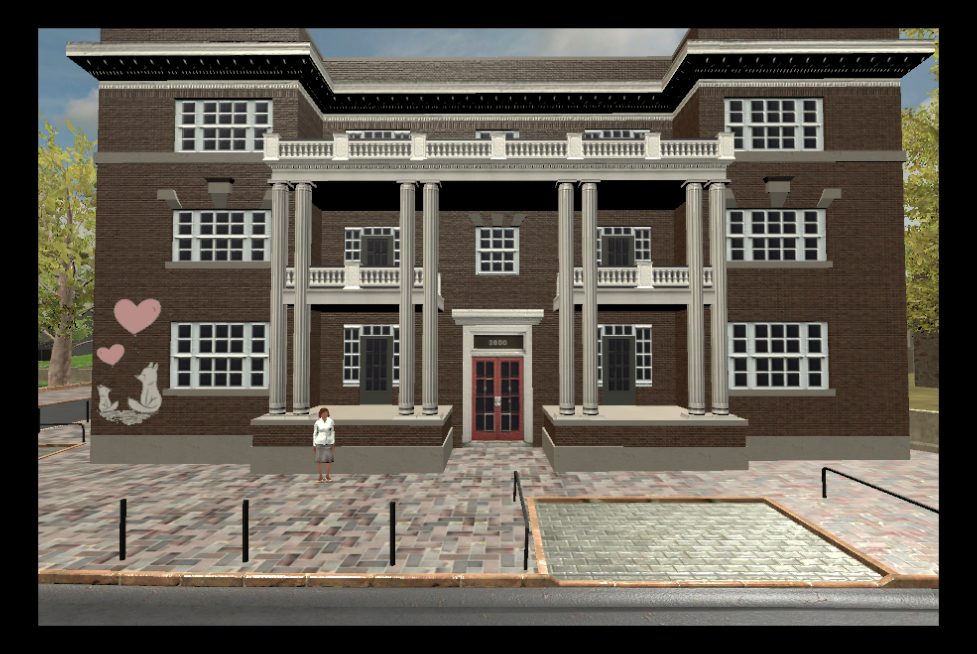
\includegraphics[width=\linewidth]{figures/starting_locations_appx/01_R(foxes)_A.PNG}
		\caption{1 (foxes) non-meaningful}
		\label{fig:01_R(foxes)_A}
	\end{subfigure}
	\begin{subfigure}[b]{0.48\linewidth}
		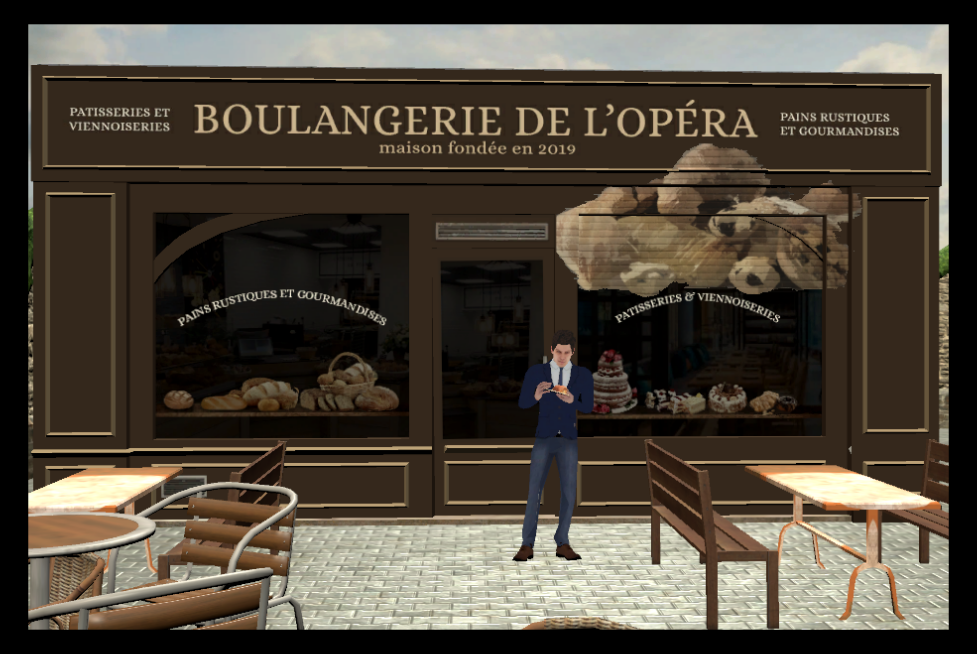
\includegraphics[width=\linewidth]{figures/starting_locations_appx/02_S(boulangerie)_A.PNG}
		\caption{2 (boulangerie) meaningful}
		\label{fig:02_S(boulangerie)_A}
	\end{subfigure}
	
	
	\begin{subfigure}[b]{0.48\linewidth}
		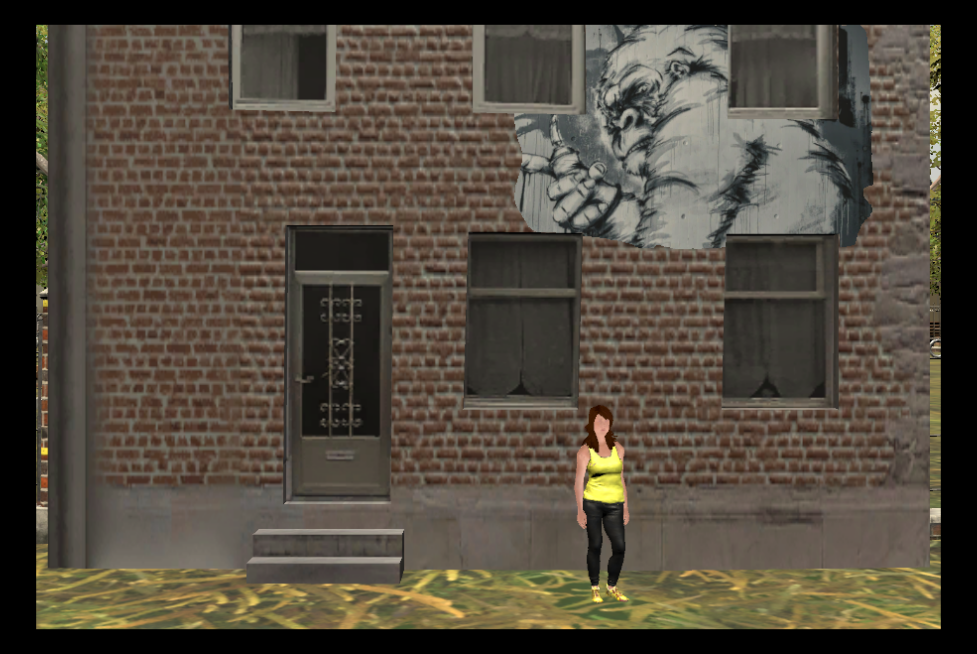
\includegraphics[width=\linewidth]{figures/starting_locations_appx/04_R(gorilla)_A.PNG}
		\caption{4 (gorilla) non-meaningful}
		\label{fig:04_R(gorilla)_A}
	\end{subfigure}
	\begin{subfigure}[b]{0.48\linewidth}
		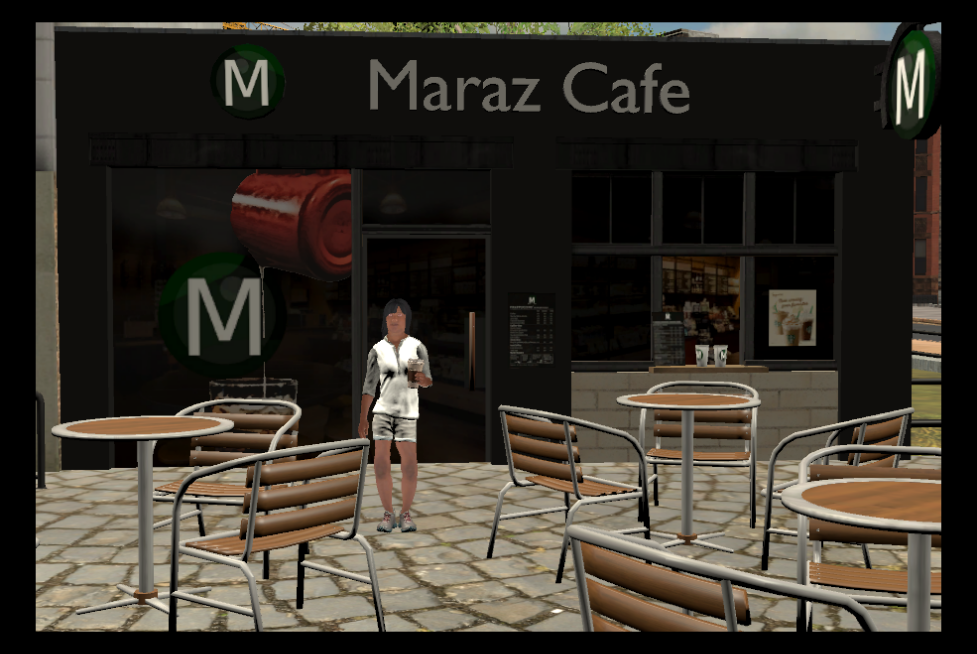
\includegraphics[width=\linewidth]{figures/starting_locations_appx/05_S(Maraz cafe)_A.PNG}
		\caption{5 (Maraz cafe) meaningful}
		\label{fig:05_S(Maraz cafe)_A}
	\end{subfigure}
	
	\caption[Starting locations 1-4]{Starting locations 1-4}
	\label{fig:starting_locations_1-4}
\end{figure}

\begin{figure}[!htb]
	\centering
	\begin{subfigure}[b]{0.48\linewidth}
		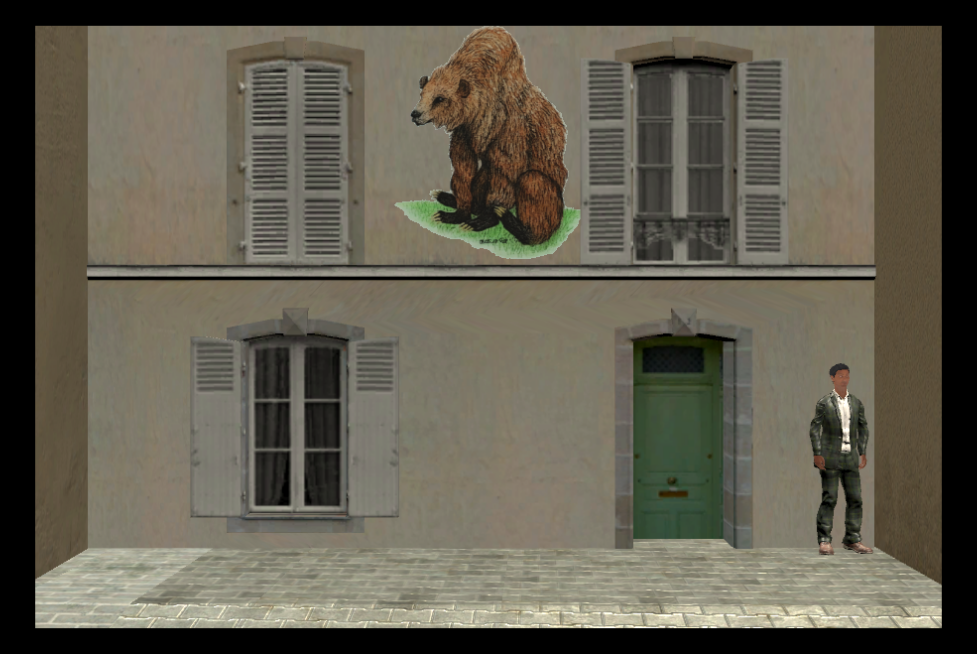
\includegraphics[width=\linewidth]{figures/starting_locations_appx/07_R(bear)_A.PNG}
		\caption{7 (bear) non-meaningful}
		\label{fig:07_R(bear)_A}
	\end{subfigure}
	\begin{subfigure}[b]{0.48\linewidth}
		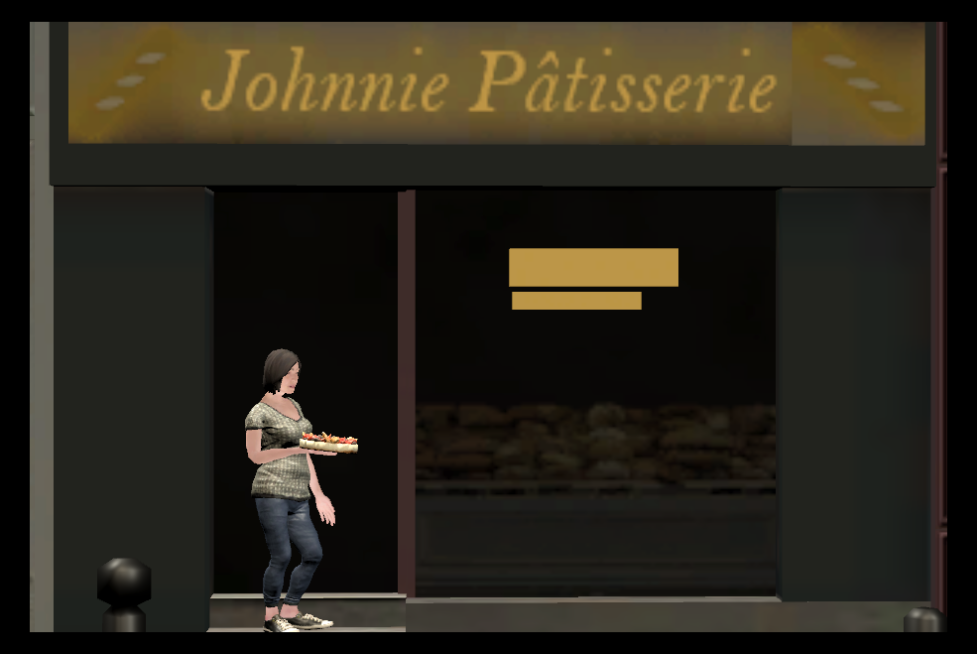
\includegraphics[width=\linewidth]{figures/starting_locations_appx/09_S(patisserie)_A.PNG}
		\caption{9 (patisserie) meaningful}
		\label{fig:09_S(patisserie)_A}
	\end{subfigure}

	\begin{subfigure}[b]{0.48\linewidth}
		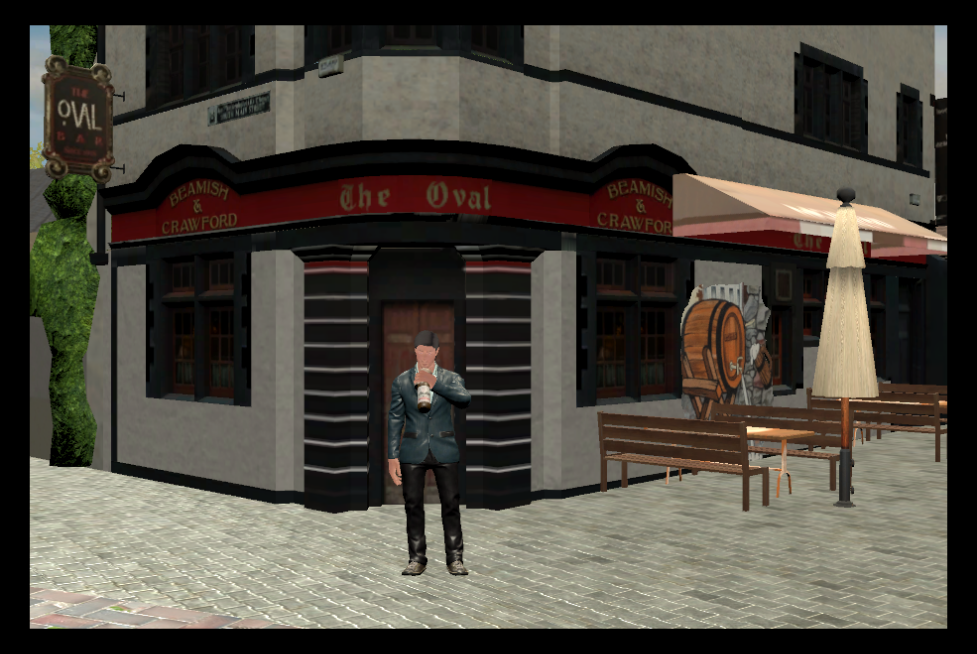
\includegraphics[width=\linewidth]{figures/starting_locations_appx/14_S(pub)_A.PNG}
		\caption{14 (pub) meaningful}
		\label{fig:14_S(pub)_A}
	\end{subfigure}
	\begin{subfigure}[b]{0.48\linewidth}
		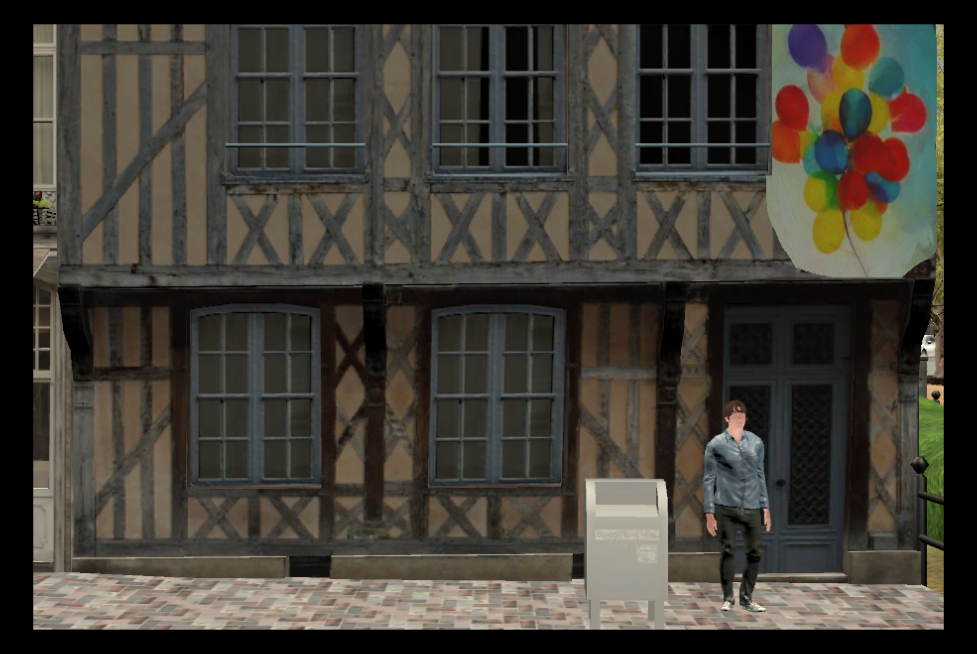
\includegraphics[width=\linewidth]{figures/starting_locations_appx/18_R(baloons)_A.PNG}
		\caption{18 (balloons) non-meaningful}
		\label{fig:18_R(baloons)_A}
	\end{subfigure}

	\begin{subfigure}[b]{0.48\linewidth}
		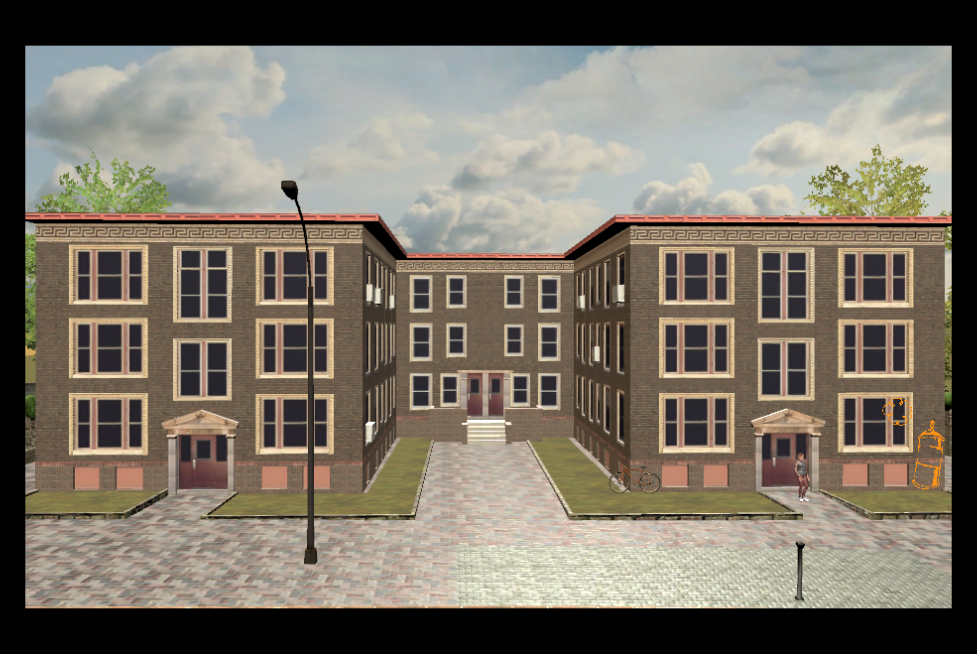
\includegraphics[width=\linewidth]{figures/starting_locations_appx/19_R(bottle spray)_A.PNG}
		\caption{19 (bottle spray) non-meaningful}
		\label{fig:19_R(bottle spray)_A}
	\end{subfigure}
	\begin{subfigure}[b]{0.48\linewidth}
		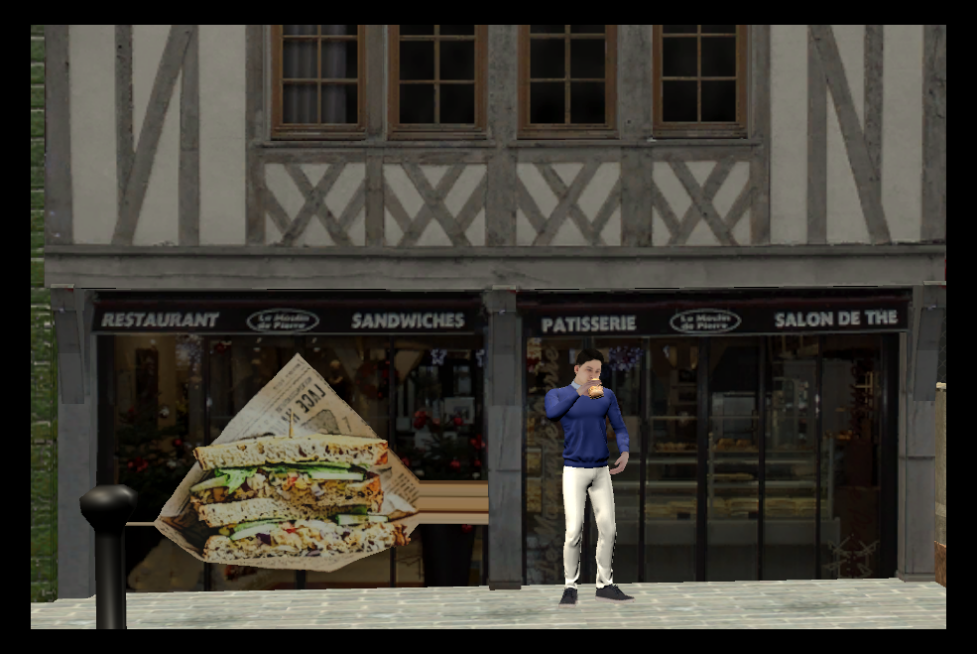
\includegraphics[width=\linewidth]{figures/starting_locations_appx/20_S(fast food)_A.PNG}
		\caption{20 (fast food) meaningful}
		\label{fig:20_S(fast food)_A}
	\end{subfigure}
	
	\begin{subfigure}[b]{0.48\linewidth}
		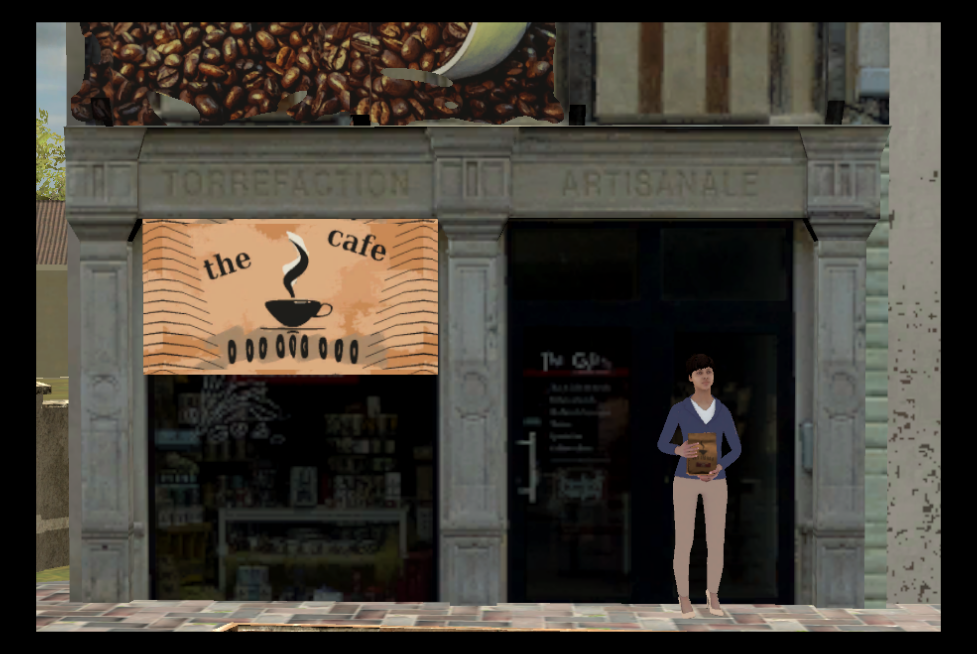
\includegraphics[width=\linewidth]{figures/starting_locations_appx/21_S(coffee store)_A.PNG}
		\caption{21 (coffee store) meaningful}
		\label{fig:21_S(coffee store)_A}
	\end{subfigure}
	\begin{subfigure}[b]{0.48\linewidth}
		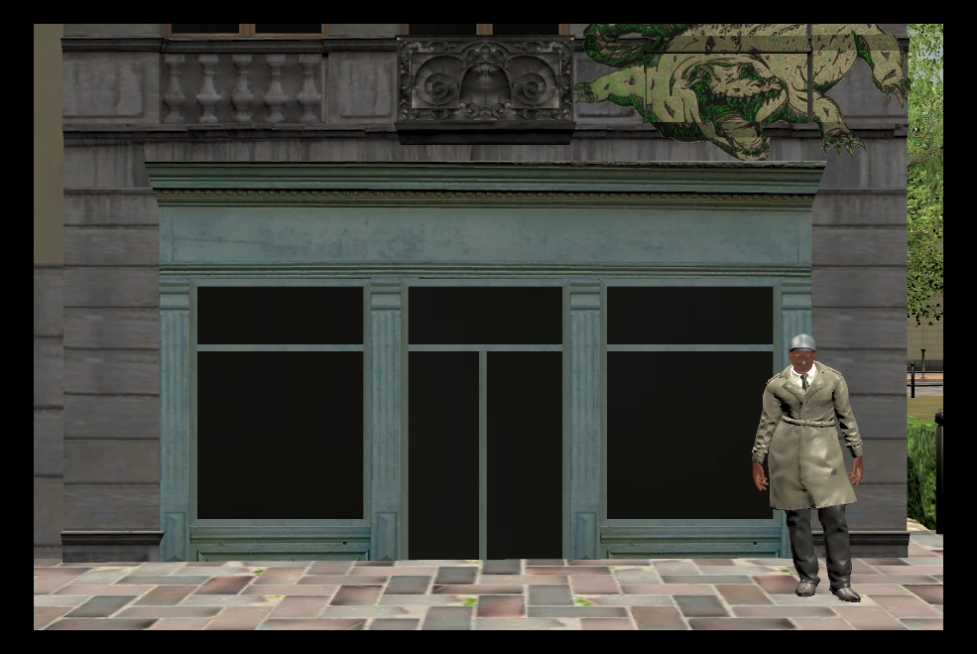
\includegraphics[width=\linewidth]{figures/starting_locations_appx/25_R(alogator)_A.PNG}
		\caption{25 (alligator) non-meaningful}
		\label{fig:25_R(alogator)_A}
	\end{subfigure}
	
	\caption[Starting locations 4-12]{Starting locations 4-12}
	\label{fig:starting_locations_4-12}
\end{figure}

\begin{figure}[!htb]
	\centering
	\begin{subfigure}[b]{0.48\linewidth}
		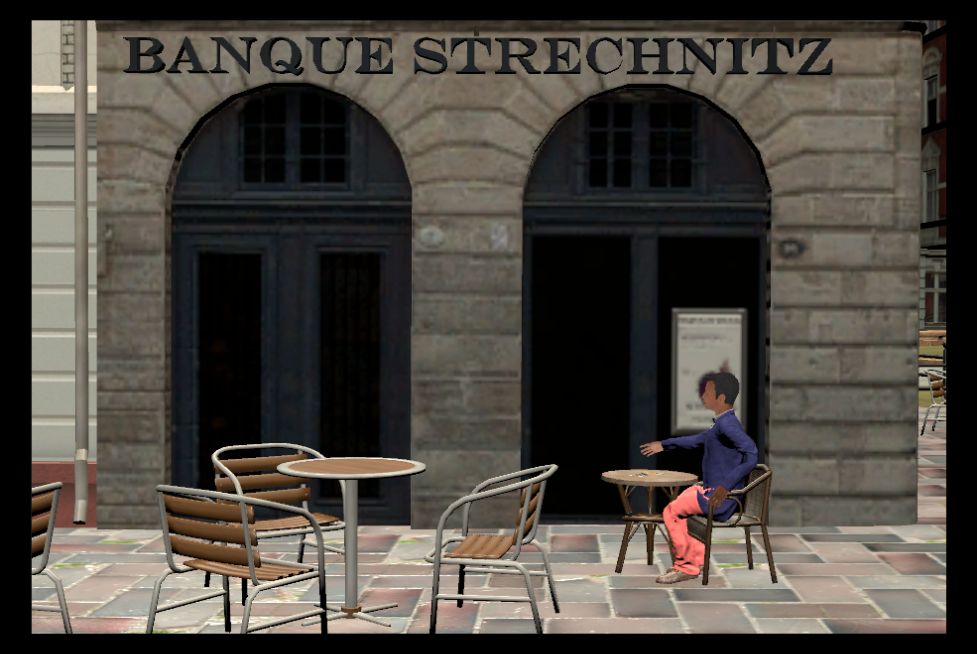
\includegraphics[width=\linewidth]{figures/starting_locations_appx/29_S(restaurant)_A.PNG}
		\caption{29 (restaurant) meaningful}
		\label{fig:29_S(restaurant)_A}
	\end{subfigure}
	\begin{subfigure}[b]{0.48\linewidth}
		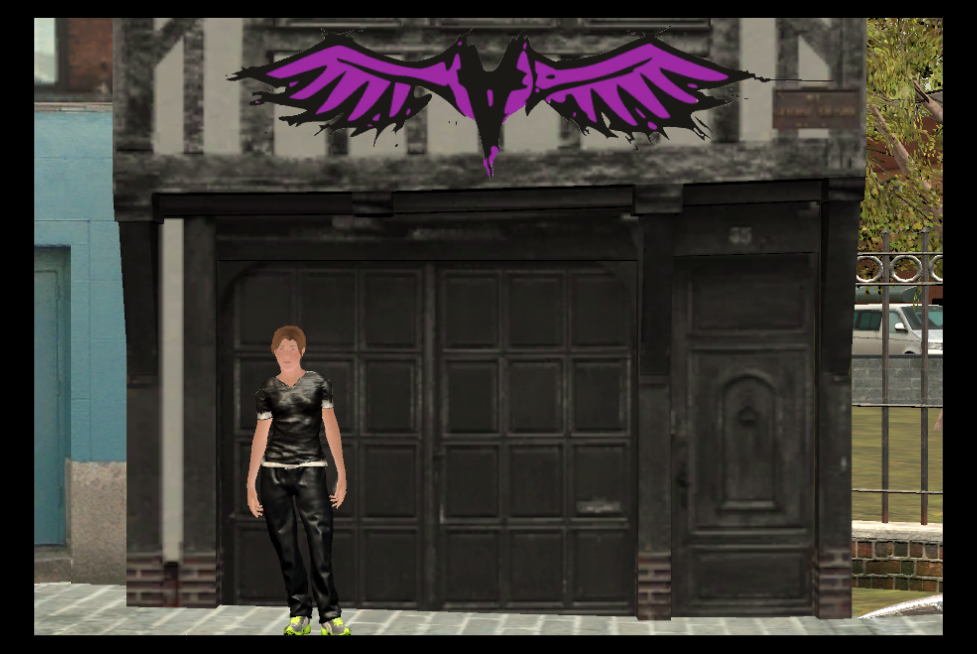
\includegraphics[width=\linewidth]{figures/starting_locations_appx/30_R(purpul bat)_A.PNG}
		\caption{30 (purple bat) non-meaningful}
		\label{fig:30_R(purpul bat)_A}
	\end{subfigure}

	\begin{subfigure}[b]{0.48\linewidth}
		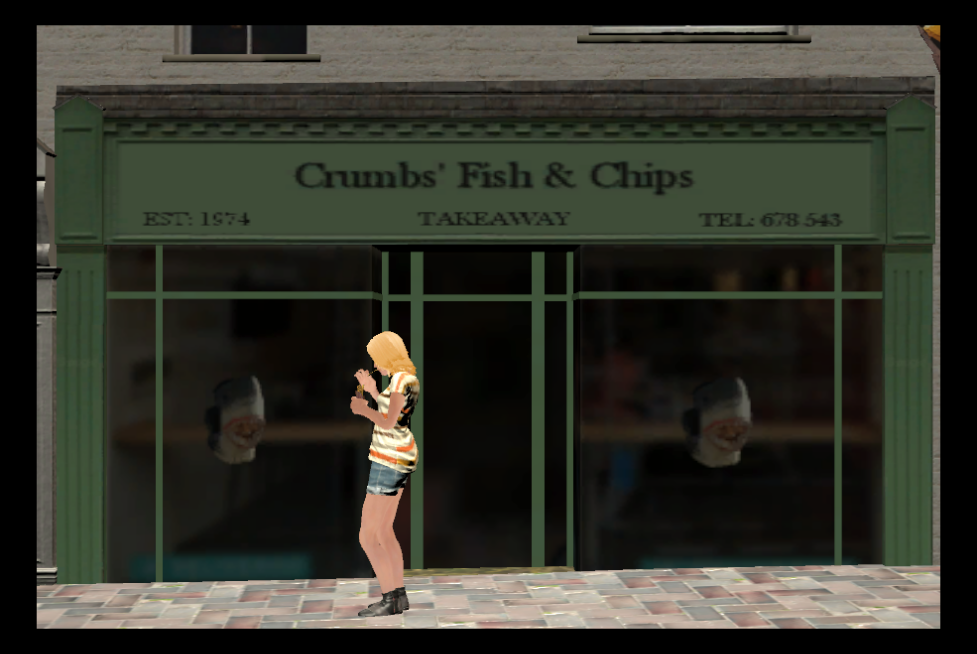
\includegraphics[width=\linewidth]{figures/starting_locations_appx/34_S(fish and chips)_A.PNG}
		\caption{34 (fish and chips) meaningful}
		\label{fig:34_S(fish and chips)_A}
	\end{subfigure}
	\begin{subfigure}[b]{0.48\linewidth}
		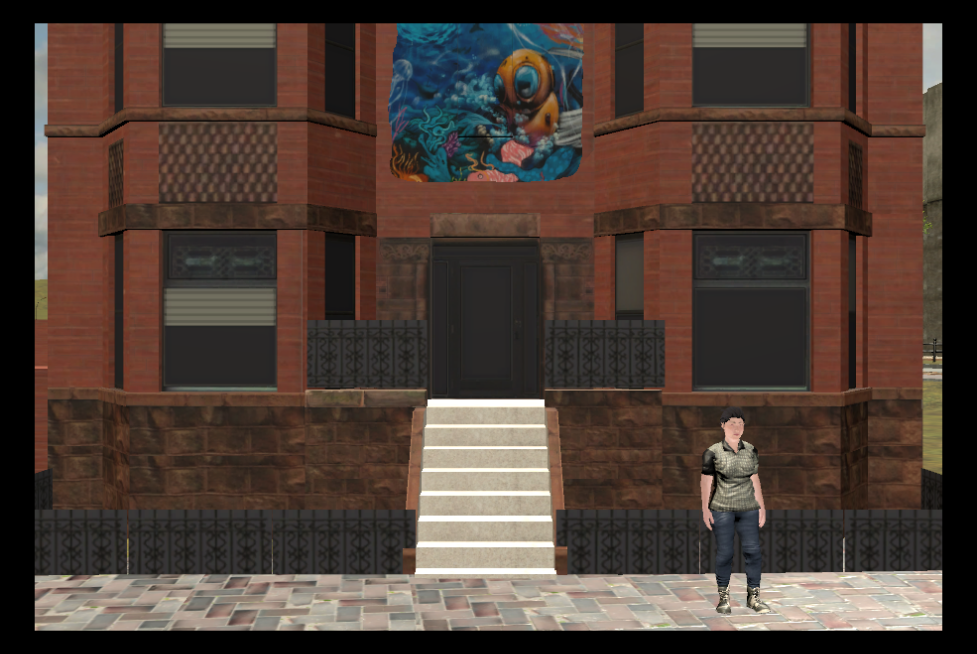
\includegraphics[width=\linewidth]{figures/starting_locations_appx/35_R(underwater)_A.PNG}
		\caption{35 (underwater) non-meaningful}
		\label{fig:35_R(underwater)_A}
	\end{subfigure}
	
	\begin{subfigure}[b]{0.48\linewidth}
		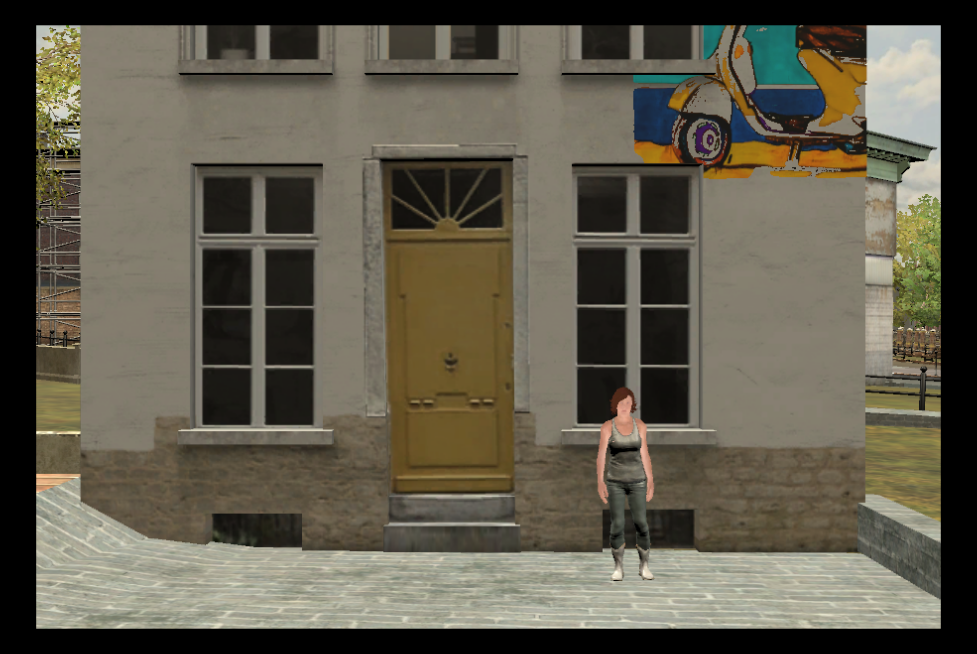
\includegraphics[width=\linewidth]{figures/starting_locations_appx/36_R(motorbike)_A.PNG}
		\caption{36 (motorbike) meaningful}
		\label{fig:36_R(motorbike)_A}
	\end{subfigure}
	\begin{subfigure}[b]{0.48\linewidth}
		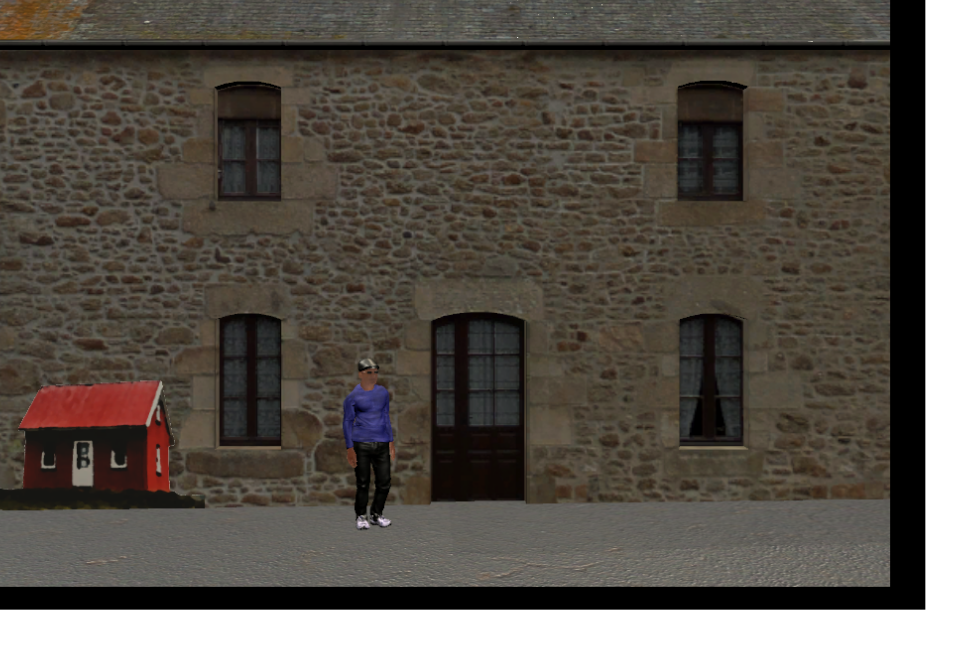
\includegraphics[width=\linewidth]{figures/starting_locations_appx/37_R(house)_A.PNG}
		\caption{37 (house) non-meaningful}
		\label{fig:37_R(house)_A}
	\end{subfigure}
	
	\begin{subfigure}[b]{0.48\linewidth}
		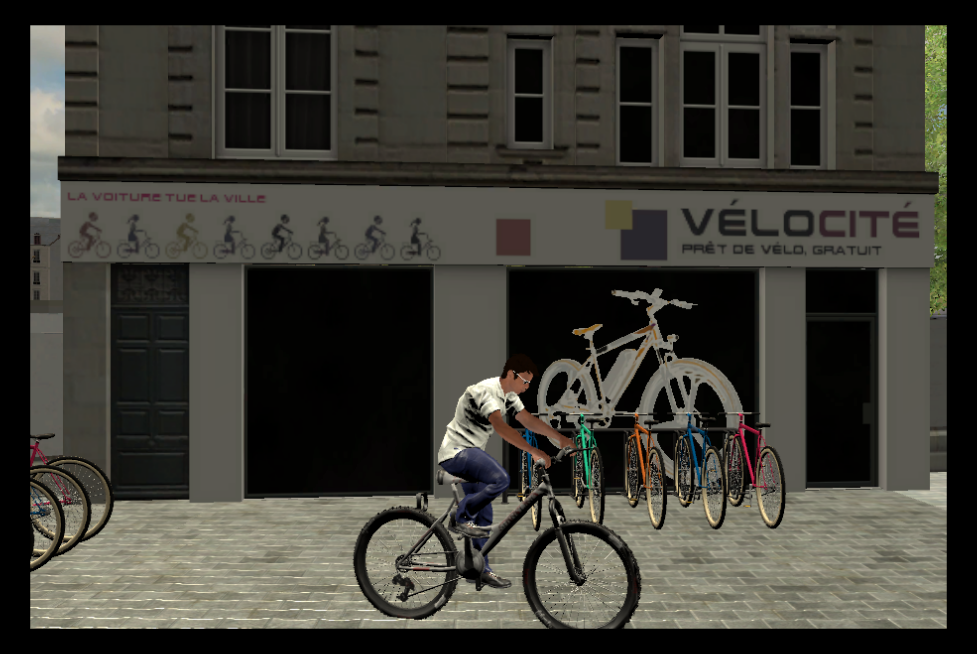
\includegraphics[width=\linewidth]{figures/starting_locations_appx/38_S(bike shop)_A.PNG}
		\caption{38 (bike shop) meaningful}
		\label{fig:38_S(bike shop)_A}
	\end{subfigure}
	\begin{subfigure}[b]{0.48\linewidth}
		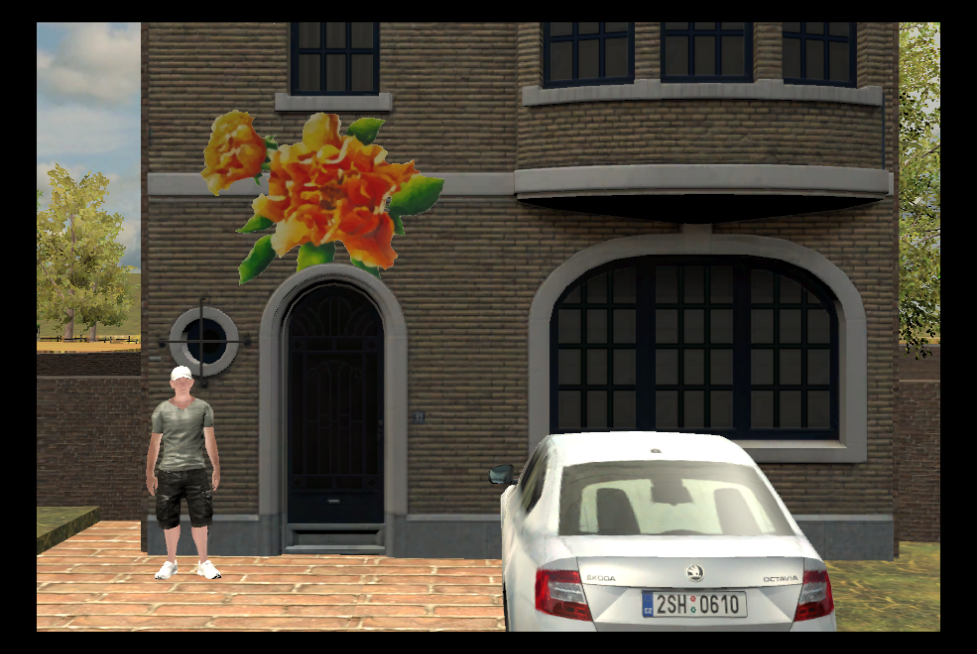
\includegraphics[width=\linewidth]{figures/starting_locations_appx/40_R(dianthus)_A.PNG}
		\caption{40 (dianthus) non-meaningful}
		\label{fig:40_R(dianthus)_A}
	\end{subfigure}
	
	\caption[Starting locations 13-20]{Starting locations 13-20}
	\label{fig:starting_locations_13-20}
\end{figure}

\begin{figure}[!htb]
	\centering
	\begin{subfigure}[b]{0.48\linewidth}
		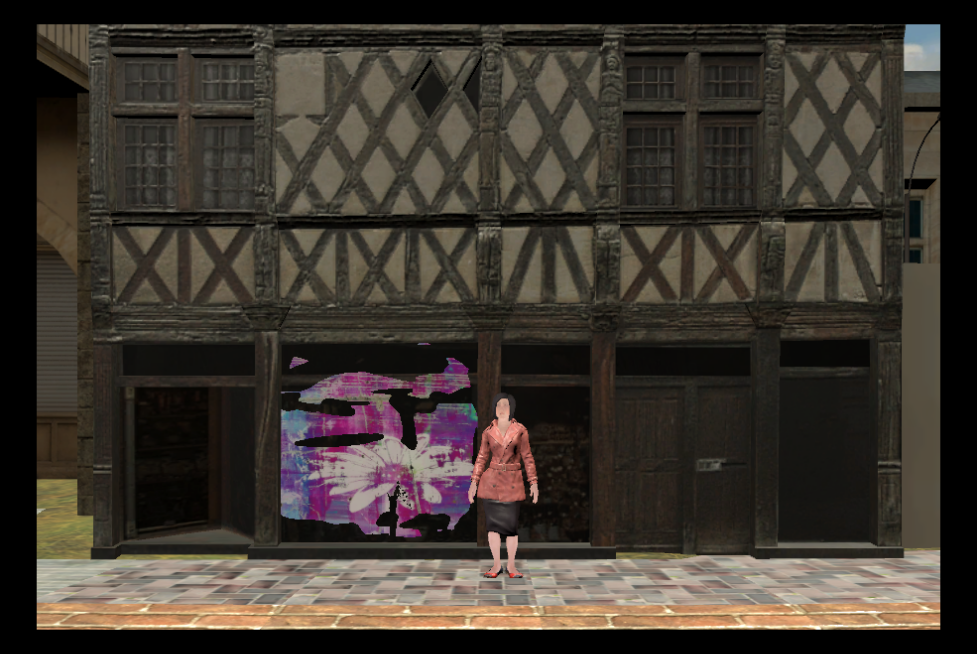
\includegraphics[width=\linewidth]{figures/starting_locations_appx/43_R(daisy)_A.PNG}
		\caption{43 (daisy) non-meaningful}
		\label{fig:43_R(daisy)_A}
	\end{subfigure}
	\begin{subfigure}[b]{0.48\linewidth}
		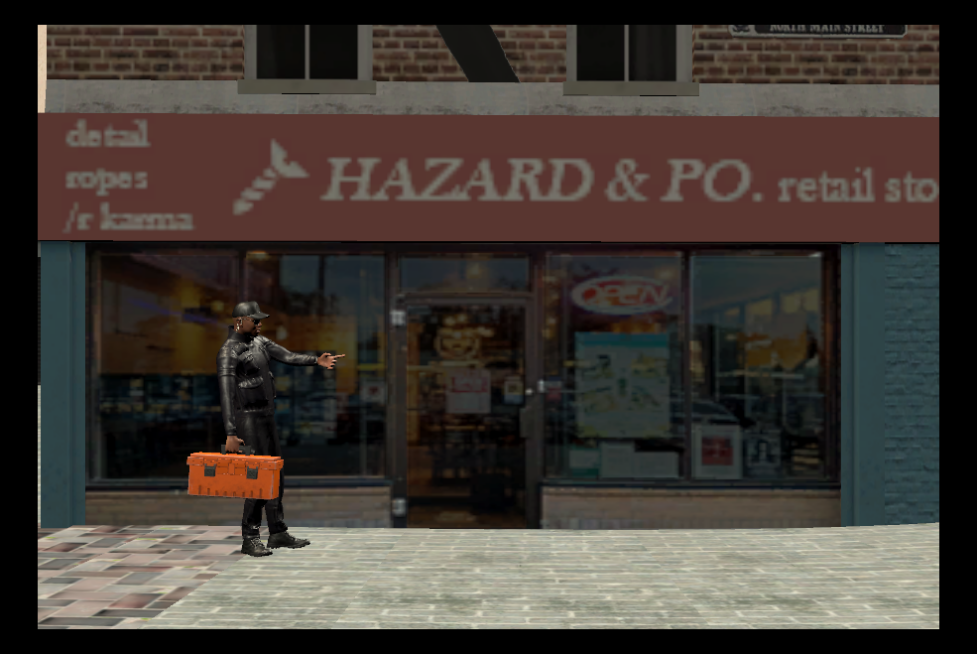
\includegraphics[width=\linewidth]{figures/starting_locations_appx/44_S(tool shop)_A.PNG}
		\caption{44 (tool shop) meaningful}
		\label{fig:44_S(tool shop)_A}
	\end{subfigure}
	
	\begin{subfigure}[b]{0.48\linewidth}
		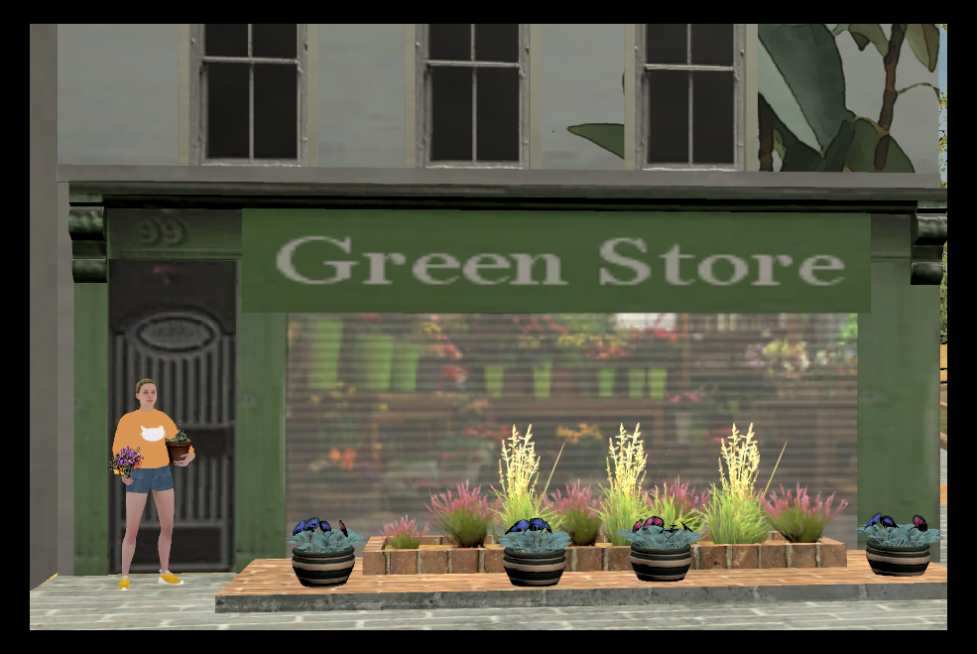
\includegraphics[width=\linewidth]{figures/starting_locations_appx/45_S(green store)_A.PNG}
		\caption{45 (green store) meaningful}
		\label{fig:45_S(green store)_A}
	\end{subfigure}
	\begin{subfigure}[b]{0.48\linewidth}
		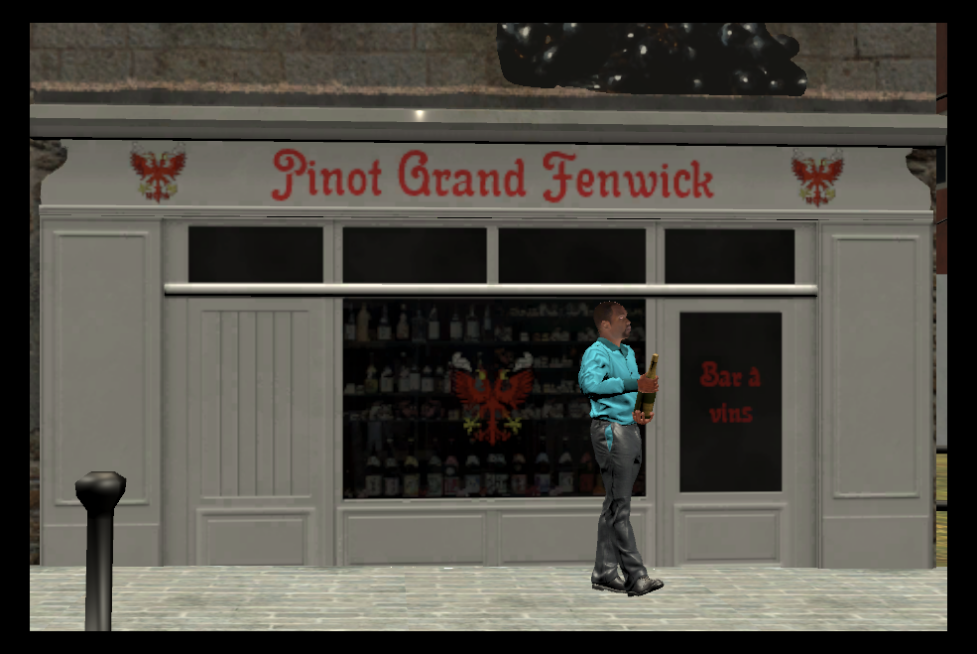
\includegraphics[width=\linewidth]{figures/starting_locations_appx/51_S(wine shop)_A.PNG}
		\caption{51 (wine shop) meaningful}
		\label{fig:51_S(wine shop)_A}
	\end{subfigure}
	
	\begin{subfigure}[b]{0.48\linewidth}
		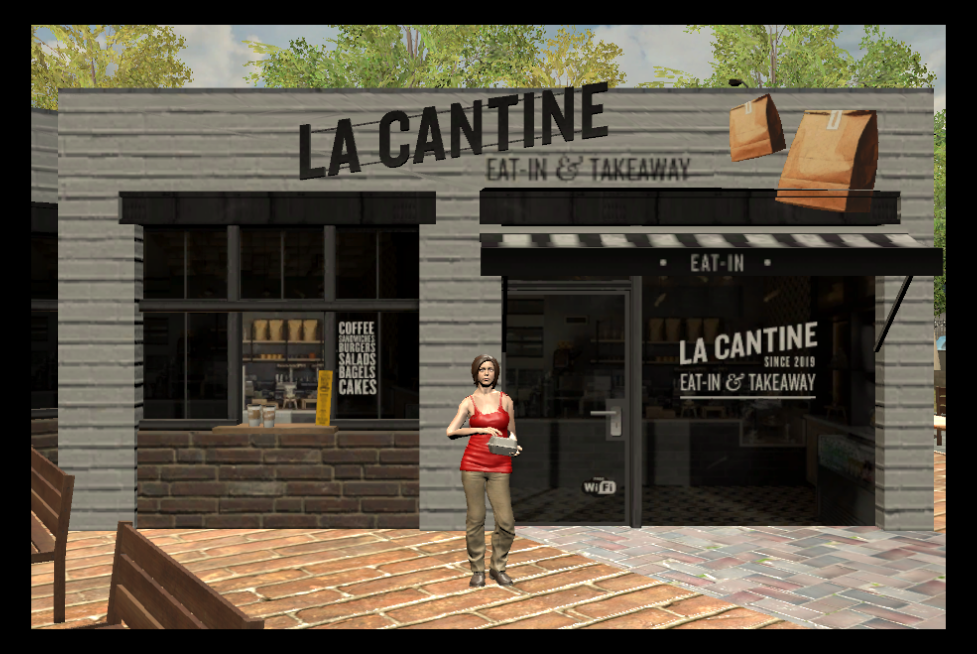
\includegraphics[width=\linewidth]{figures/starting_locations_appx/52_S(la cantine)_A.PNG}
		\caption{52 (la cantine) meaningful}
		\label{fig:52_S(la cantine)_A}
	\end{subfigure}
	\begin{subfigure}[b]{0.48\linewidth}
		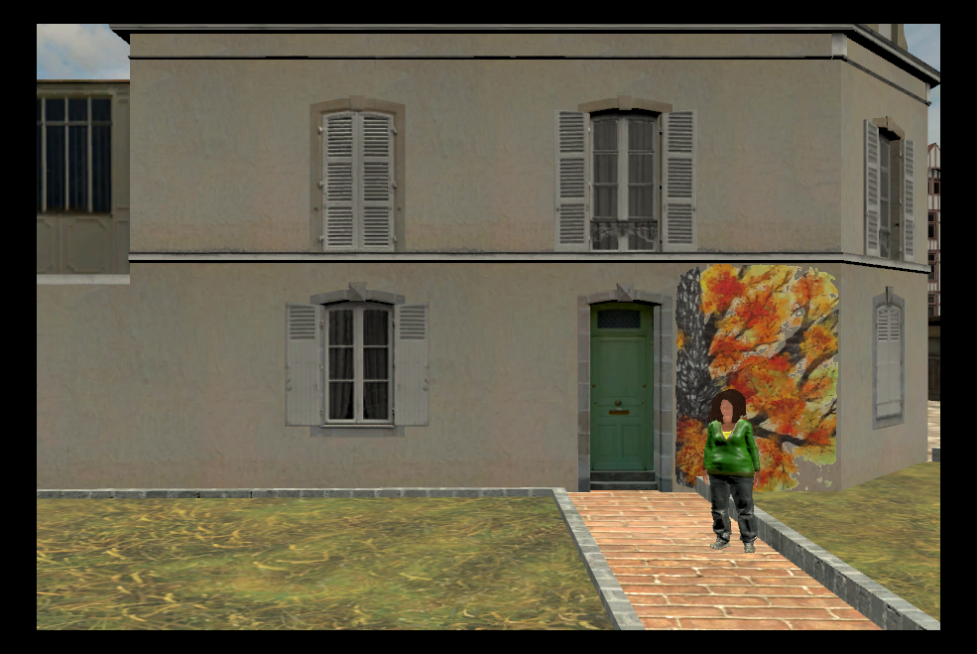
\includegraphics[width=\linewidth]{figures/starting_locations_appx/54_R(tree)_A.PNG}
		\caption{54 (tree) non-meaningful}
		\label{fig:54_R(tree)_A}
	\end{subfigure}
	
	\begin{subfigure}[b]{0.48\linewidth}
		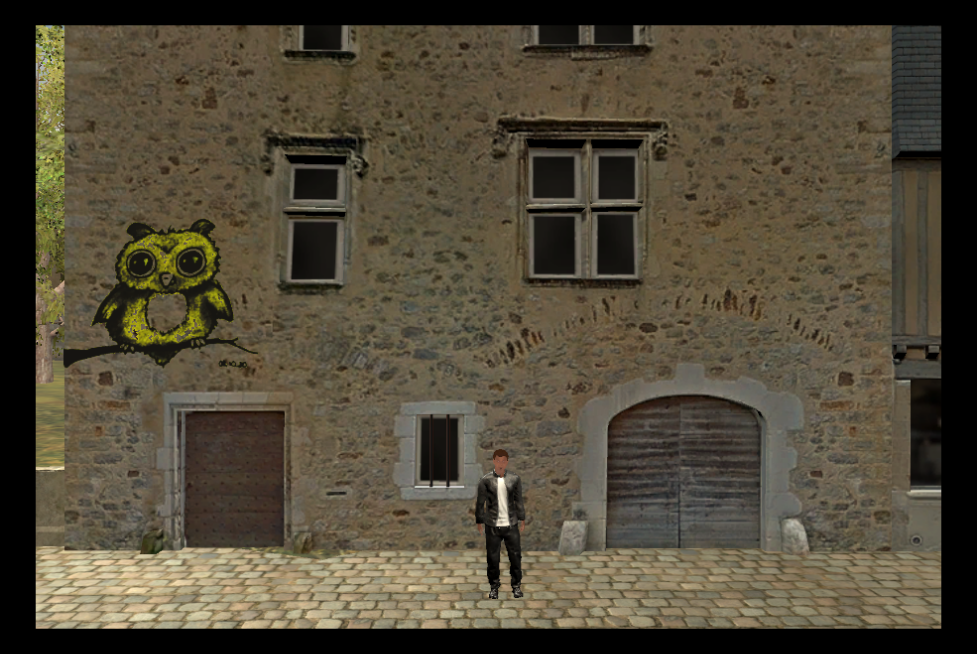
\includegraphics[width=\linewidth]{figures/starting_locations_appx/55_R(bird)_A.PNG}
		\caption{55 (bird) non-meaningful}
		\label{fig:55_R(bird)_A}
	\end{subfigure}
	\begin{subfigure}[b]{0.48\linewidth}
		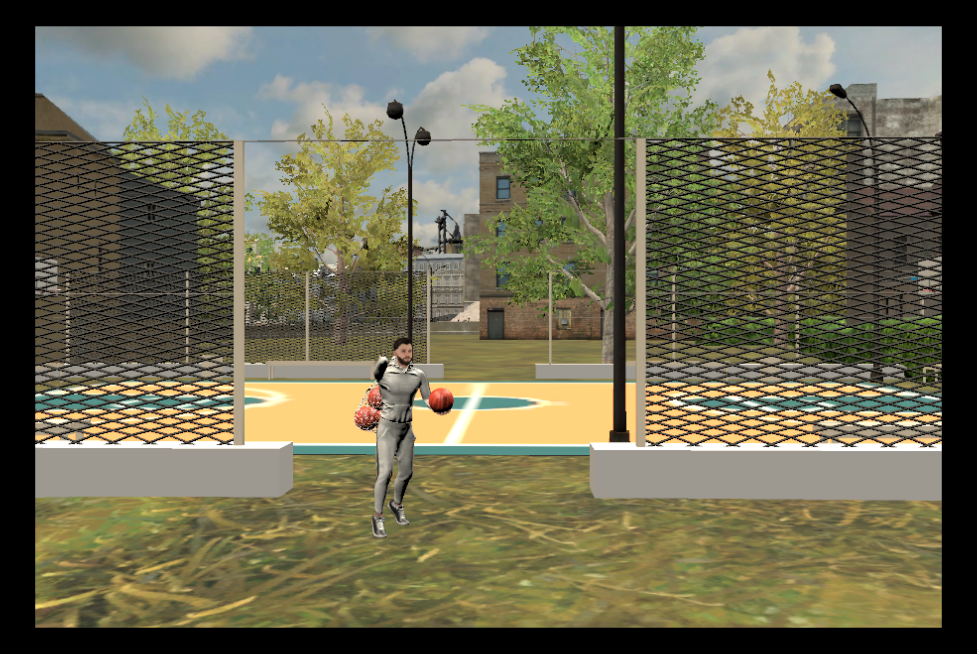
\includegraphics[width=\linewidth]{figures/starting_locations_appx/58_basketball court_A.PNG}
		\caption{58 (basketball court) meaningful}
		\label{fig:58_basketball court_A}
	\end{subfigure}
	
	\caption[Starting locations 21-28]{Starting locations 21-28}
	\label{fig:starting_locations_21-28}
\end{figure}


\chapter{Additional plots}\label{appx:plots}

\begin{figure}[!htb]
	\centering
	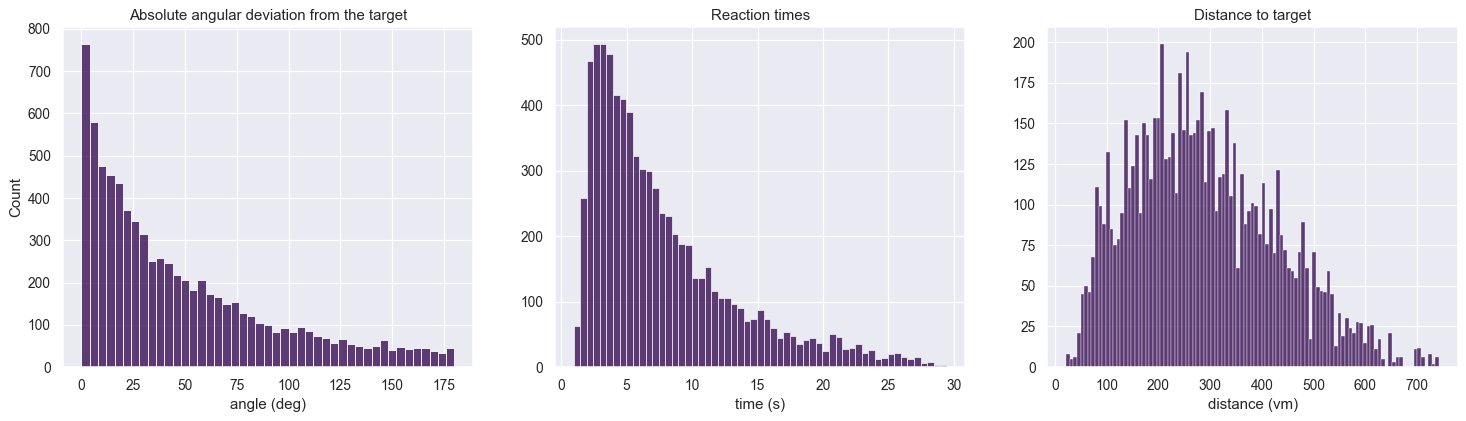
\includegraphics[width=160mm]{figures/ard_hist.png}
	\caption[Distribution of absolute angular deviation from the target, reaction times and distance to target]{Distribution of absolute angular deviation from the target, reaction times and distance to target. "vm" stands for virtual meter.}
	\label{fig:ard_hist}
\end{figure}

\begin{figure}[!htb]
	\centering
	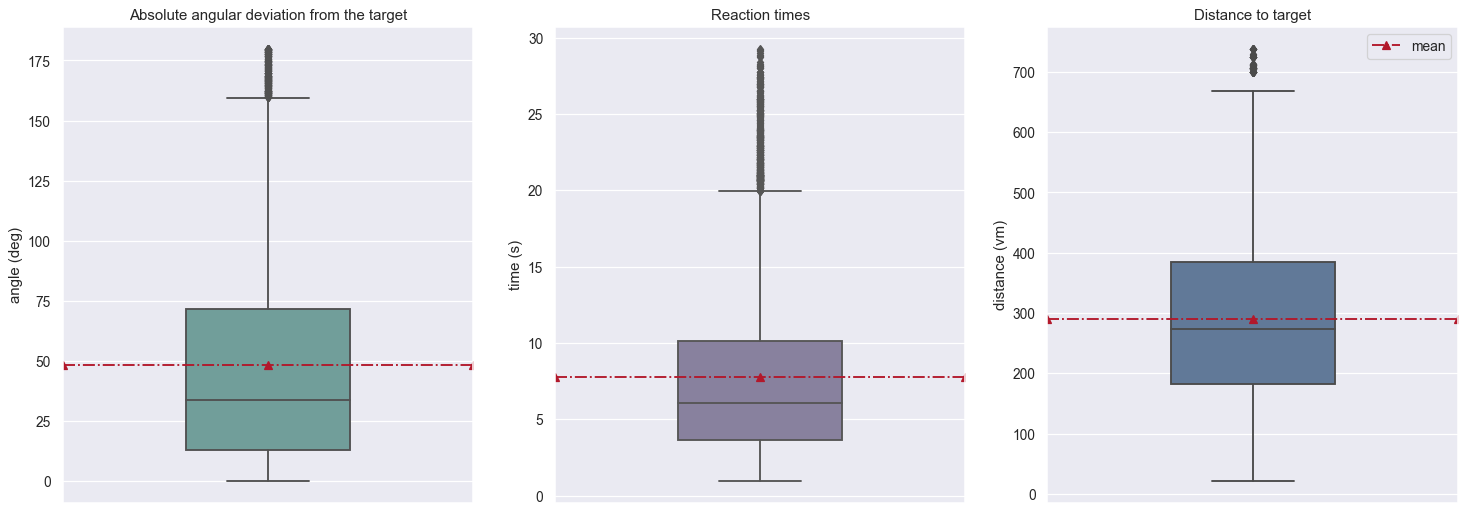
\includegraphics[width=160mm]{figures/ard_box.png}
	\caption[Box plot of absolute angular deviation from the target, reaction times and distance to target]{Box plot of absolute angular deviation from the target, reaction times and distance to target. "vm" stands for virtual meter.}
	\label{fig:ard_box}
\end{figure}


\begin{figure}[!htb]
	\centering
	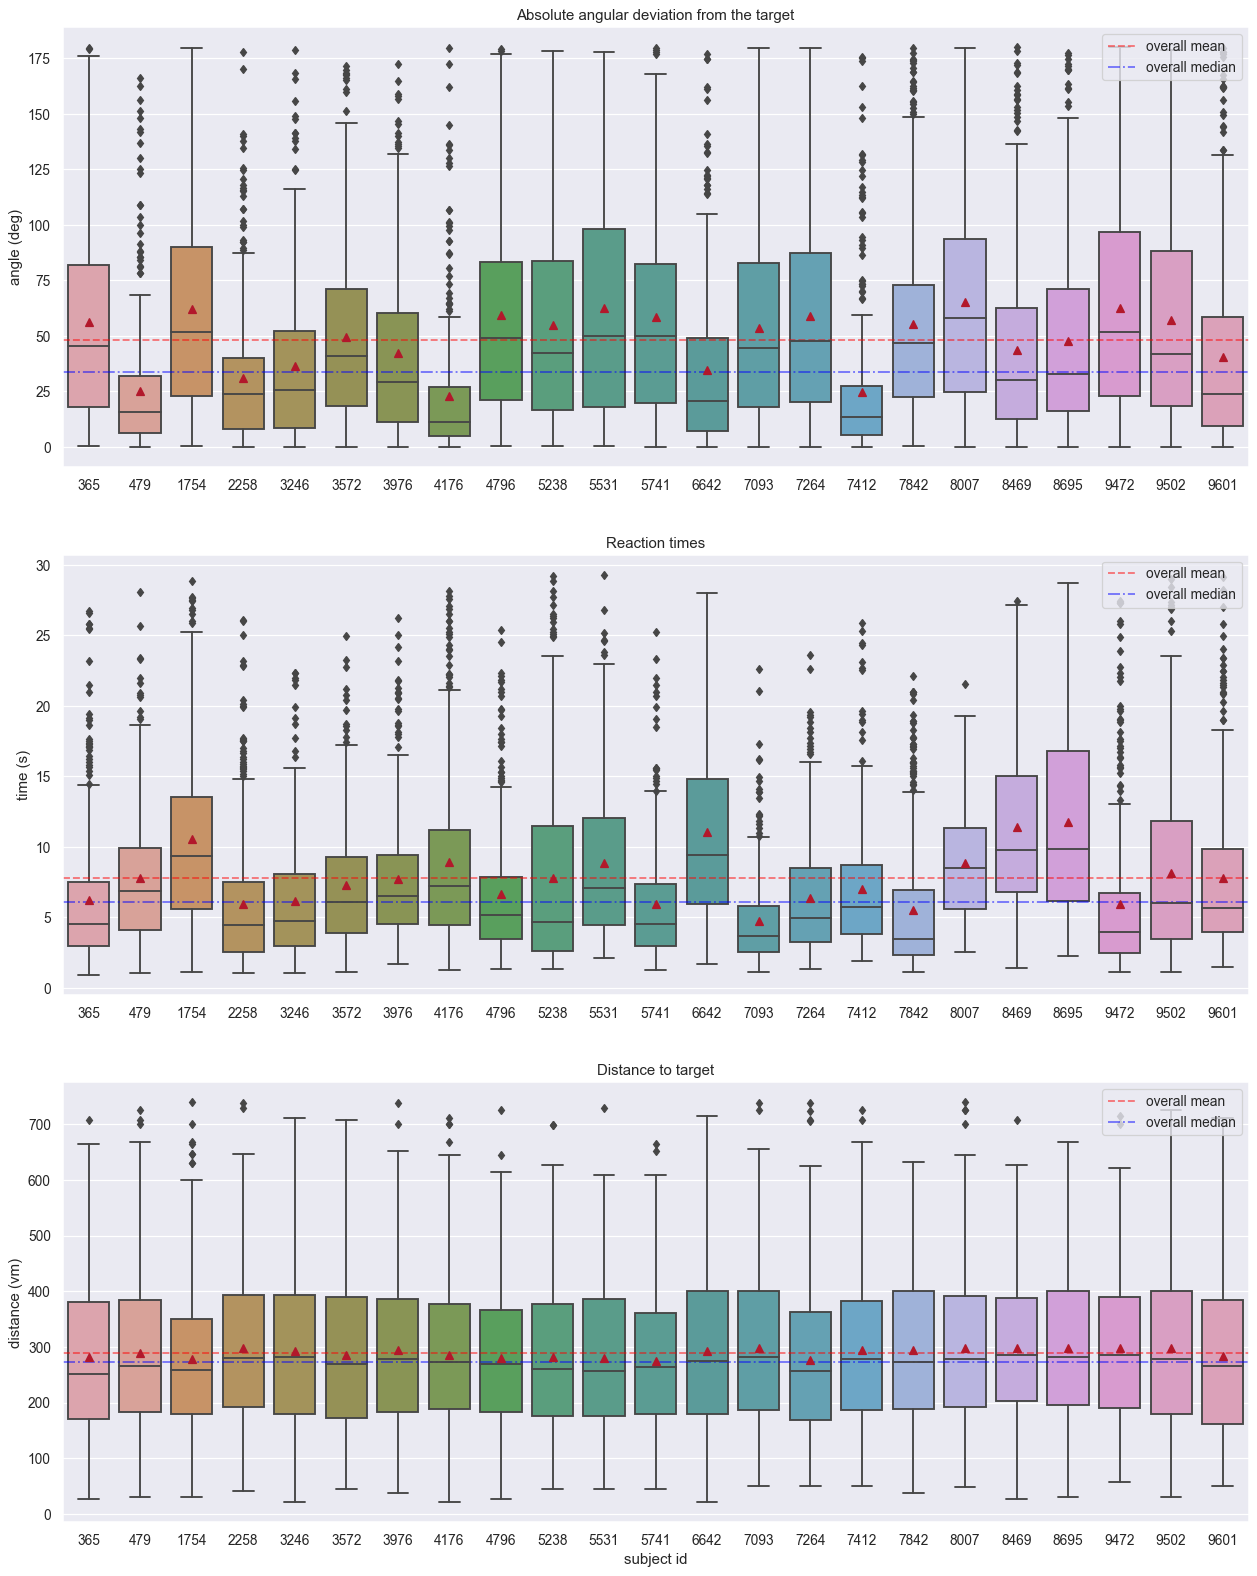
\includegraphics[width=160mm]{figures/ard_by_subject_23.png}
	\caption[Box plot by subject]{Absolute angular deviation, reaction times and distance to target by subject. Red triangles depict the mean and "vm" stands for virtual meter.}
	\label{fig:ard_by_subject_23}
\end{figure}


\begin{figure}[!htb]
	\centering
	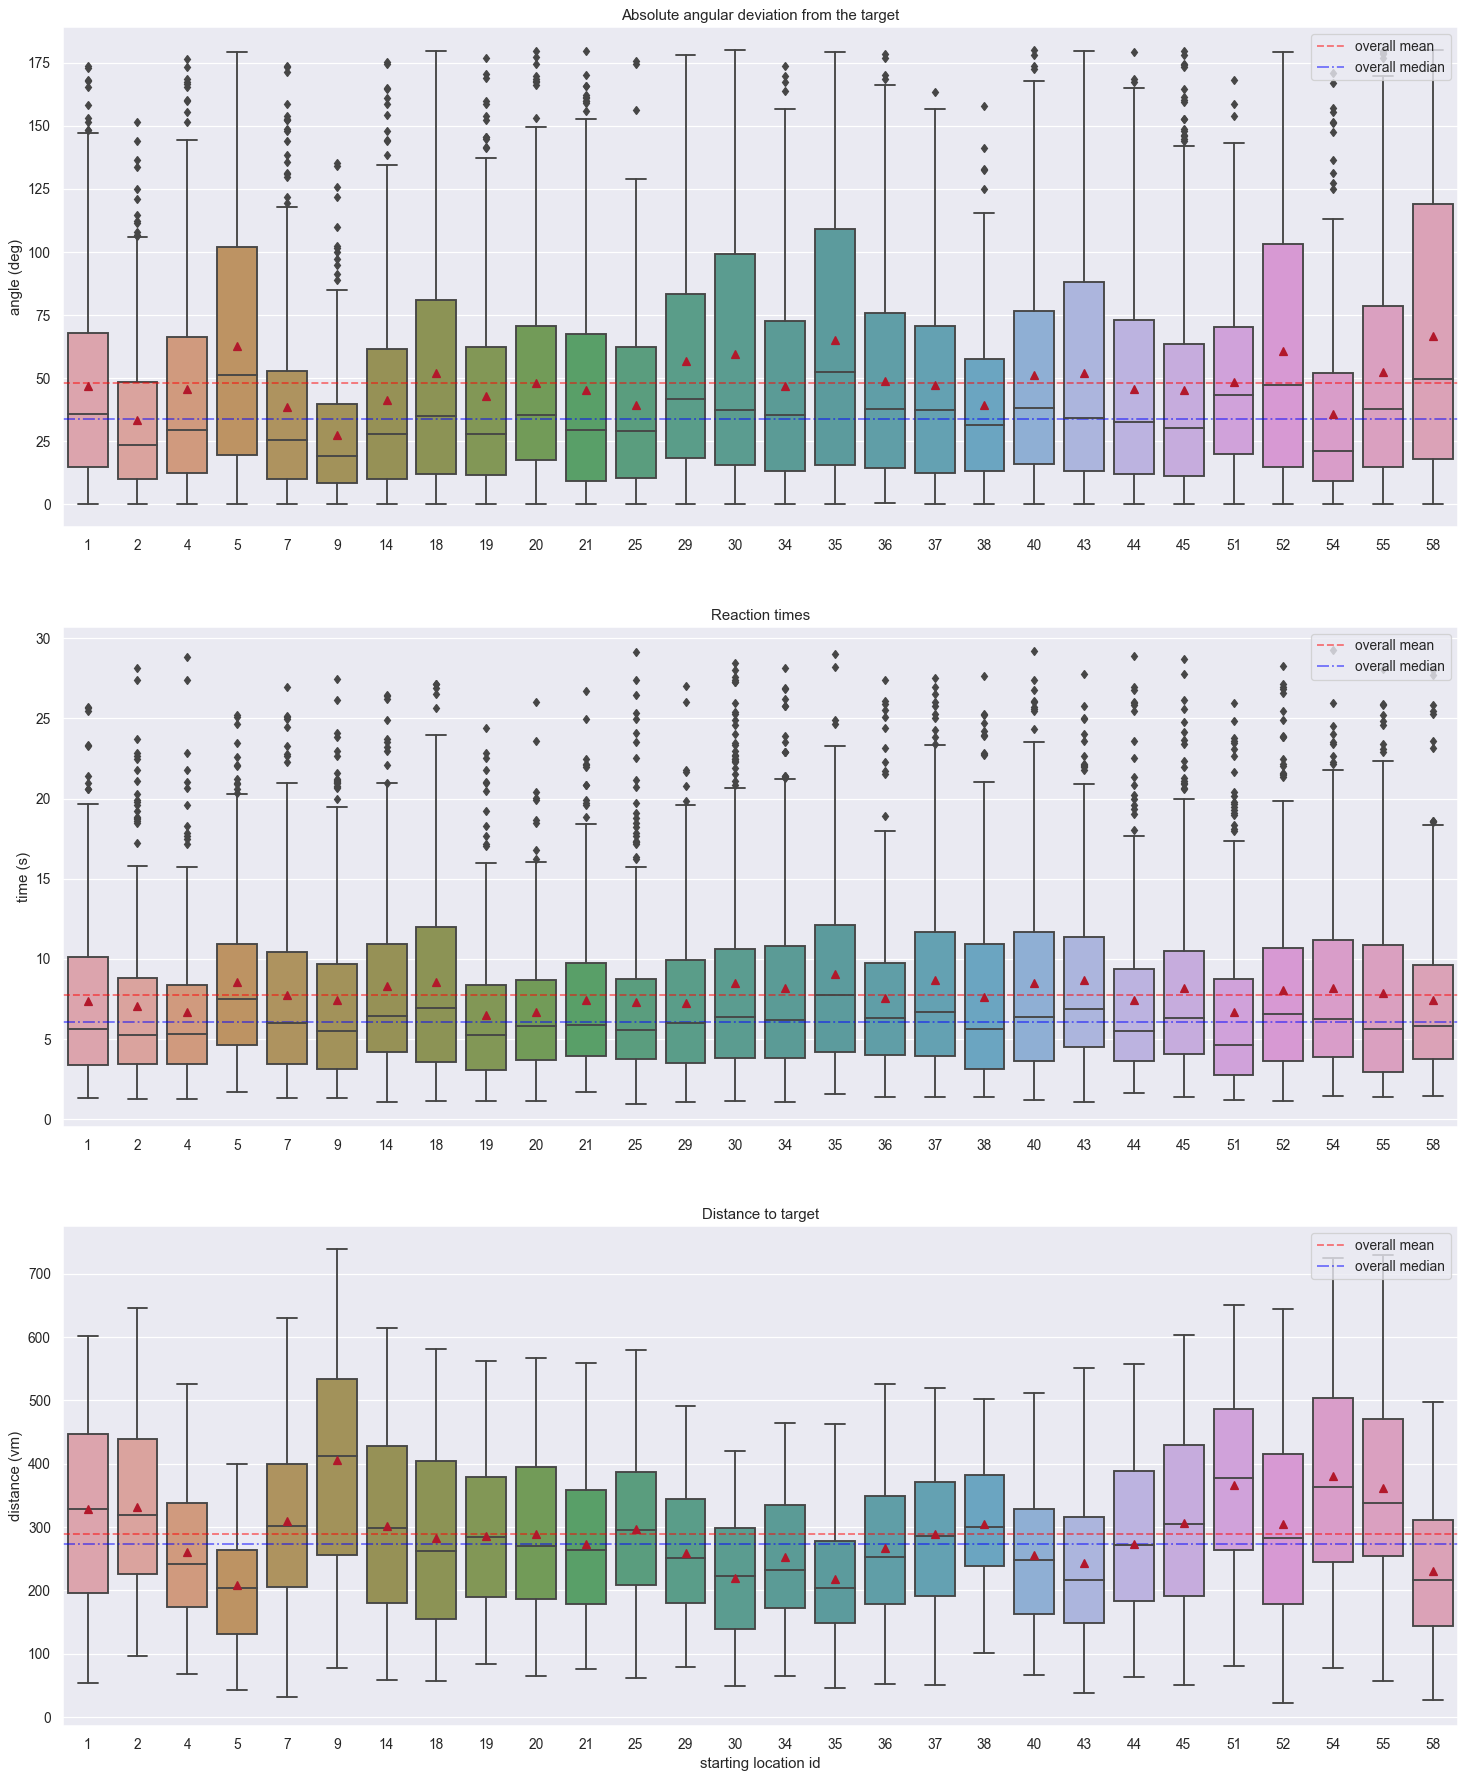
\includegraphics[width=160mm]{figures/ard_by_starting_locations_23.png}
	\caption[Box plot per starting location]{Absolute angular deviation, reaction times and distance to target at each starting location. Red triangles depict the mean and "vm" stands for virtual meter.}
	\label{fig:ard_by_starting_locations_23}
\end{figure}

\begin{figure}[!htb]
	\centering
	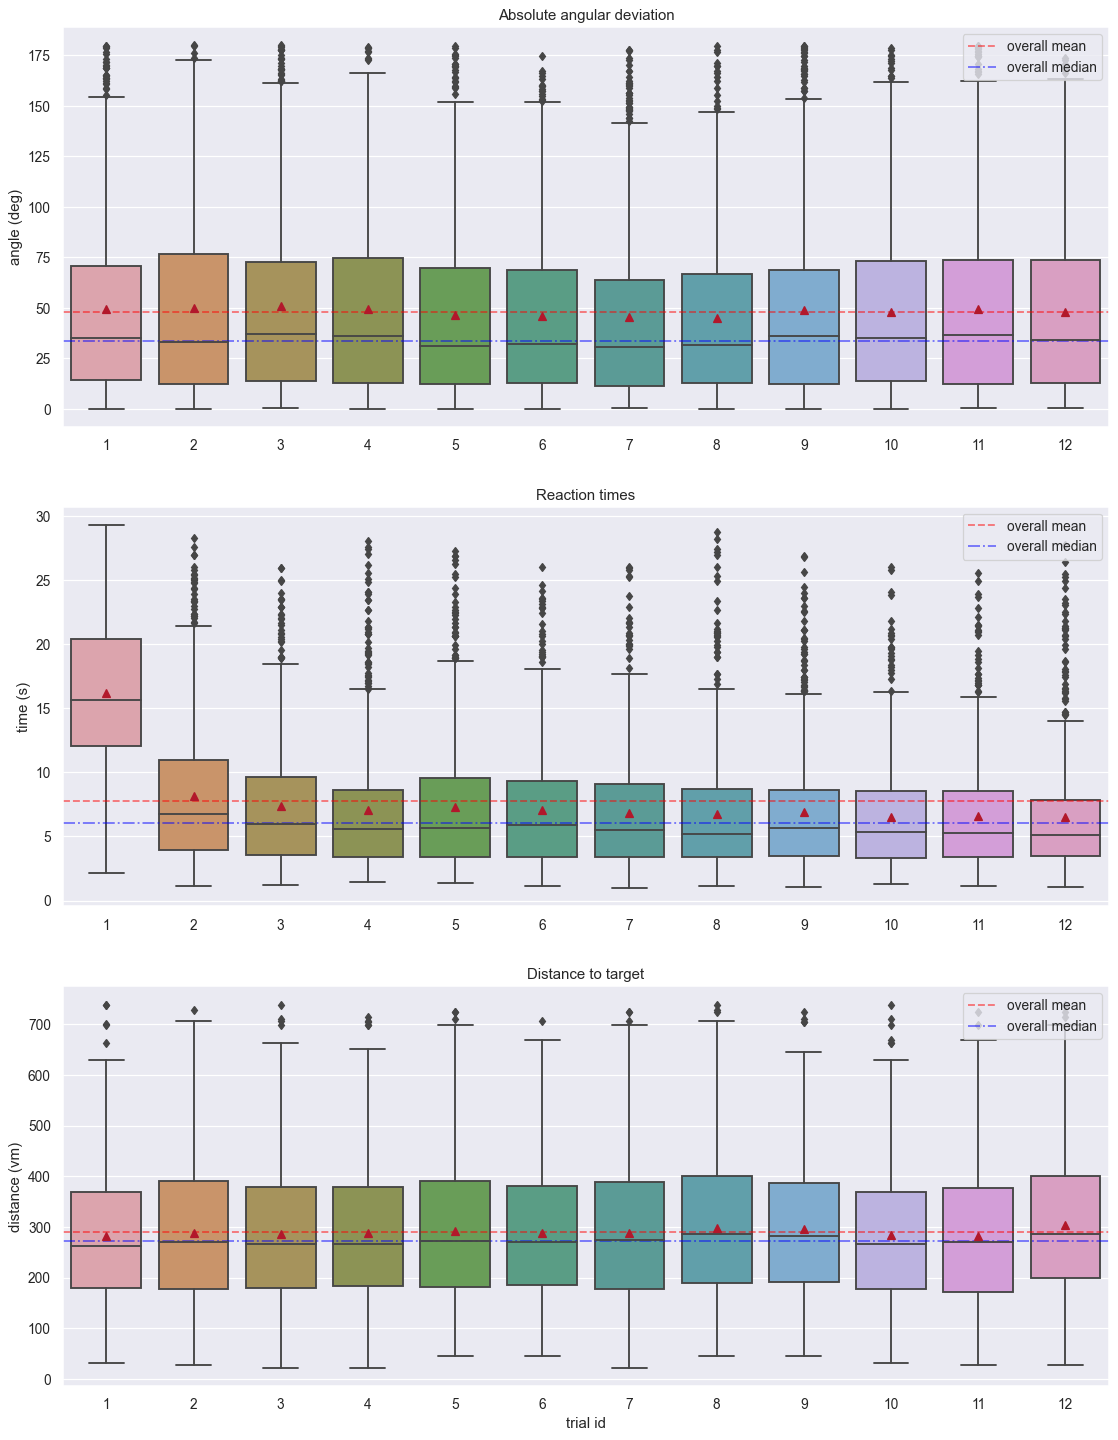
\includegraphics[width=140mm]{figures/ard_per_trial_order_of_each_starting_location_23.png}
	\caption[Box plot per consecutive trials at each starting location]{Absolute angular deviation, reaction times and distance to target per consecutive trials at each starting location. Red triangles depict the mean and "vm" stands for virtual meter.}
	\label{fig:ard_per_trial_order_of_each_starting_location_23}
\end{figure}

\begin{figure}[!htb]
	\centering
	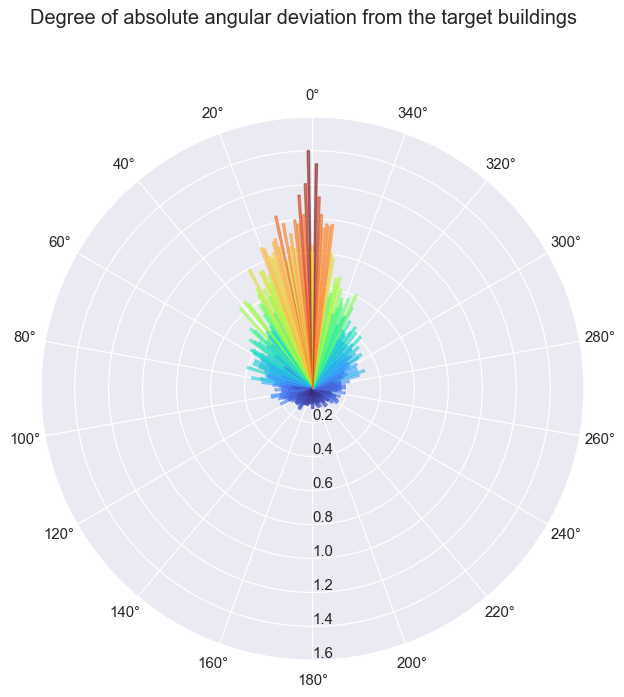
\includegraphics[width=80mm]{figures/deviation_degree_all_23.png}
	\caption[Angular deviation from the target in all trials]{Angular deviation from the target in all trials}
	\label{fig:deviation_degree_all_23}
\end{figure}

\begin{figure}[!htb]
	\centering
	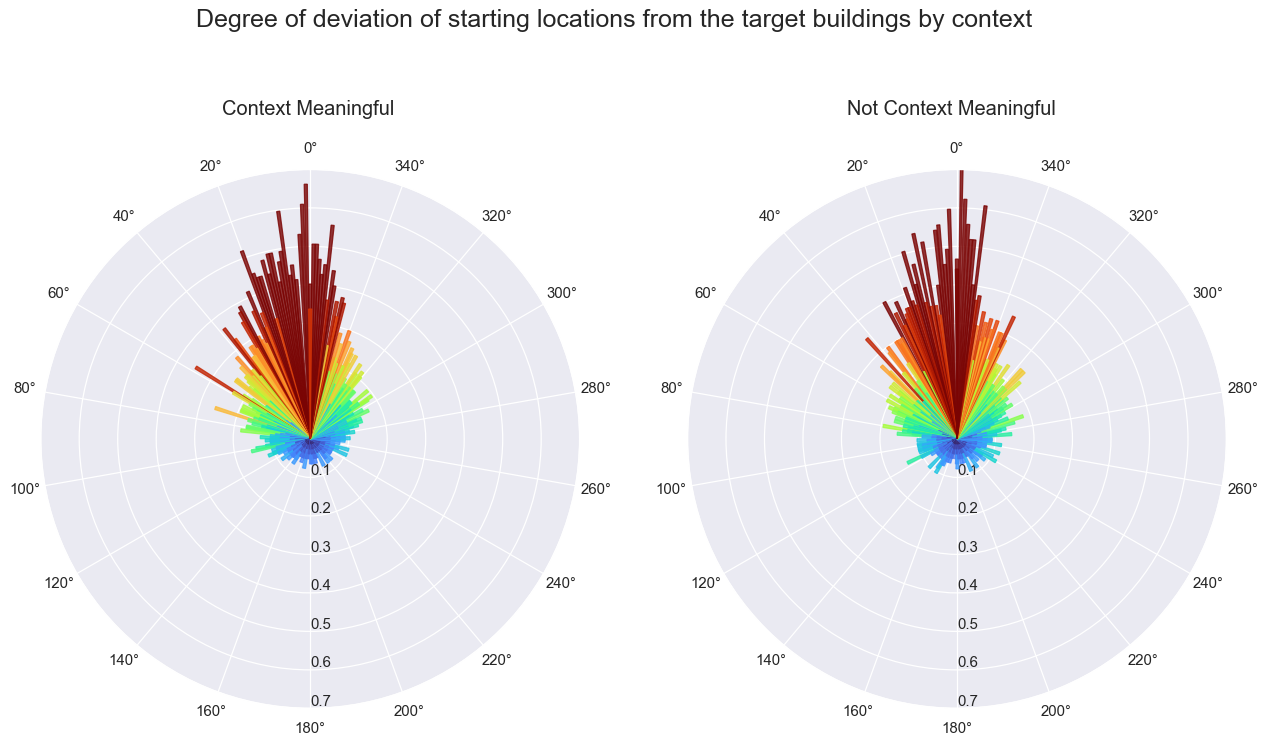
\includegraphics[width=140mm]{figures/by_context_deviation_for_starting_locations_23.png}
	\caption[Angular deviation of starting locations from the target by meaningfulness]{Angular deviation of starting locations from the target by meaningfulness.}
	\label{fig:by_context_deviation_for_starting_locations_23}
\end{figure}

\begin{figure}[!htb]
	\centering
	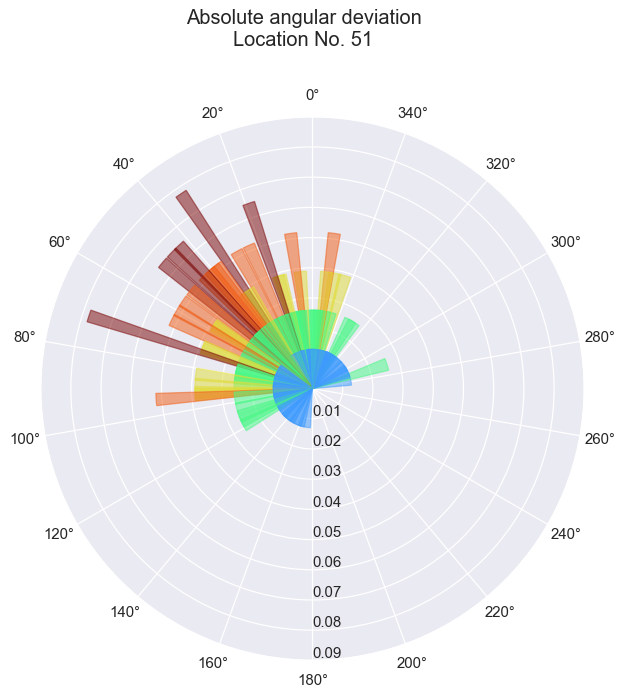
\includegraphics[width=80mm]{figures/deviation_degrees_loc_nr_51_23.png}
	\caption[Absolute angular deviation of the fastest starting location]{Absolute angular deviation of the fastest starting location, location No. 51.}
	\label{fig:angle_fastest_loc}
\end{figure}

\begin{figure}[!htb]
	\centering
	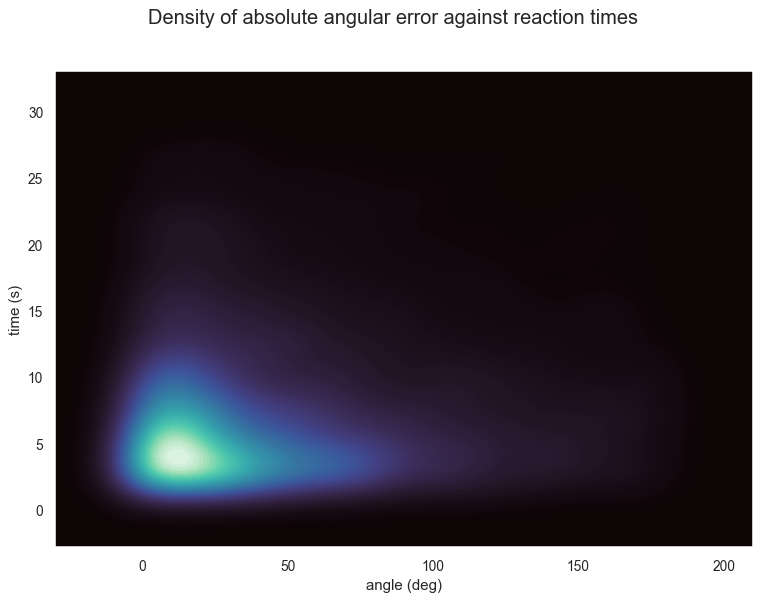
\includegraphics[width=100mm]{figures/density_angular_error_reaction_time_23.png}
	\caption[Density of absolute angular error against reaction times]{Density of absolute angular error against reaction times.}
	\label{fig:density_angular_error_reaction_time_23}
\end{figure}


\chapter{Forms}\label{appx:forms}

\begin{center}
	\LARGE{\textbf{Einverständniserklärung}} \\
\end{center}


\textbf{Titel der Studie:} Untersuchung des Effektes von menschlichen Avataren auf räumliches Lernen und räumliche Navigation in einer virtuellen Stadt unter Einbeziehung des Blickverhaltens \\

\textbf{Zweck der Studie:} Das Ziel des vorliegenden Forschungsprojekts ist es, den Effekt von menschlichen Avataren auf das Lernen durch aktive Navigation in einer virtuellen Stadt zu untersuchen. Zu diesem Zweck werden wir menschliche Avatare strategisch neben Gebäuden innerhalb einer virtuellen Stadt platzieren. Auf Basis der erhobenen Daten werden wir evaluieren, ob die Teilnehmer sich die Teile der Stadt, in denen wir Avatare platziert haben, besser merken konnten. \\

\textbf{Projektleitung:} Prof. Dr. Peter König, Dr. med. Sabine König, Prof. Dr. Gordon Pipa, Tracy Sánchez (Lic.), Institut für Kognitionswissenschaften, Wachsbleiche 27, 49082 Osnabrück \\


Sehr geehrte Studienteilnehmerin, sehr geehrter Studienteilnehmer,
hiermit bitten wir Sie um Ihre Einwilligung zur Teilnahme an dem oben genannten Forschungsvorhaben und zur Nutzung Ihrer personenbezogenen Daten, wie sie Ihnen in der Probandeninformation und der Aufklärung näher erläutert worden sind. \\

\begin{center}
	\large{\textbf{I. Allgemeines}} \\
\end{center}

Hiermit erkläre ich, \_\_\_\_\_\_\_\_\_\_\_, geboren am \_\_\_\_\_\_\_\_\_, dass ich durch die Projektleitung mündlich und schriftlich über das Wesen, die Bedeutung, die Risiken und Folgen der wissenschaftlichen Untersuchungen im Rahmen der o.g. Studie informiert und aufgeklärt wurde und ausreichend Gelegenheit hatte, meine Fragen mit der Projektleitung zu klären. \\

Mir ist bekannt, dass ich das Recht habe, meine Einwilligung jederzeit ohne Angabe von Gründen und ohne nachteilige Folgen für mich zurückzuziehen. Mir ist bekannt, dass meine Daten nach Abschluss der Datenerhebung nur in anonymisierter Form gespeichert, analysiert und veröffentlicht werden. Dies führt dazu, dass ein späteres Löschen meiner Daten nicht mehr möglich ist, da die Daten nicht mehr meiner Person zugeordnet werden können. \\

Ich habe eine Kopie der schriftlichen Studieninformation und der Einwilligungs-erklärung erhalten. \\

Ich erkläre, dass ich freiwillig bereit bin, an der wissenschaftlichen Studie, die für mich aus 5 wiederholten Erkundungen in der virtuellen Stadt „Westbrück“, die jeweils 45 Minuten dauern werden und einer Testsession in der virtuellen Umgebung, die ungefähr 120 Minuten dauern wird, teilzunehmen. Die Erkundungs- und Testsessions finden jeweils an unterschiedlichen Tagen statt. \\

Insbesondere erkläre ich mich damit einverstanden, \\

1.     dass die in der Studie aufgenommenen Daten in anonymisierter Form gespeichert und analysiert werden, auch auf elektronischen Datenträgern; \\
\_\_\_\_\_\_\_\_ (Initialen Proband) \\

2.     dass meine persönlichen Daten zu Zwecken der Vergütung und Dokumentation gespeichert werden. Diese persönlichen Daten werden nur in Papierform und nicht mit den experimentellen Daten verbunden aufgehoben. \\
\_\_\_\_\_\_\_\_ (Initialen Proband) \\

3.     dass an dieser Studie folgende beteiligte Wissenschaftler Zugang zu den erhobenen anonymisierten experimentellen Daten zum Zweck der Durchführung und wissenschaftlichen Verwertung der Studie haben: Prof. Dr. Peter König, Dr. med. Sabine König, Prof. Dr. Gordon Pipa, Tracy Sánchez, Institut für Kognitionswissenschaften, Universität Osnabrück;  \\
\_\_\_\_\_\_\_\_ (Initialen Proband) \\

4.     dass die Studienergebnisse und die Studiendaten in anonymisierter Form, die nach heutigem Stand der Technik keinen Rückschluss auf meine Person zulässt, veröffentlicht werden; die Veröffentlichung kann zum Beispiel in einer wissenschaftlichen Zeitschrift oder im Internet erfolgen;  \\
\_\_\_\_\_\_\_\_ (Initialen Proband) \\

5.     dass meine Daten, im Sinne der guten wissenschaftlichen Praxis, in anonymisierter Form der Öffentlichkeit über eine Creative Commons Lizenz (CC0) zugänglich gemacht werden;  \\
\_\_\_\_\_\_\_\_ (Initialen Proband) \\

6.     dass ich aktiv eine virtuelle Stadt erkunde. Anschließend werde ich Orientierungstests in der virtuellen Stadt durchführen. Während des Navigationstrainings werde ich eine virtuelle Realitätsbrille tragen. Die Messungen finden in einem Labor des Instituts für Neurobiopsychologie der Universität Osnabrück statt  \\
\_\_\_\_\_\_\_\_ (Initialen Proband) \\

7. dass die in der Studie aufgenommenen Daten entsprechend der Empfehlung durch die DFG mindestens 10 Jahre lang aufbewahrt werden. \\
\_\_\_\_\_\_\_\_ (Initialen Proband) \\

\begin{center}
	\large{\textbf{II. Ausschlusskriterien, Verhaltensregeln}} \\
\end{center}

\textbf{II.1 Ausschlusskriterien} \\

Ich versichere, den mir vorgelegten Anamnesebogen wahrheitsgemäß ausgefüllt zu haben. Mir ist bewusst, dass während des Trainings in der virtuellen Stadt „Seekrankheits-“ ähnliche Symptome („Bewegungsübelkeit“) wie Schwindel und Übelkeit auftreten können. Des Weiteren ist mir bewusst, dass das Tragen der virtuellen Brille ein Druckgefühl bis hin zu leichten Kopfschmerzen und ein Verspannungsgefühl im Nacken auslösen kann.  \\

\textbf{II.2 Zustimmung zur Einhaltung von Verhaltensregeln} \\

Ich wurde vor der Durchführung der Studie darauf hingewiesen, dass ich vor oder während der Untersuchung auftretendes körperliches oder psychisches Unwohlsein der Projektleitung unverzüglich mitzuteilen habe. Ich wurde zusätzlich informiert, dass ich jederzeit während des Experimentes eine Pause einlegen darf. \\

\begin{center}
	\large{\textbf{III. Datenschutzrechtliche Einwilligungserklärung}} \\
\end{center}


Einblick in die anonymisierten Daten durch Dritte findet statt: \\

Ich bin damit einverstanden, dass die erhobenen Daten in anonymisierter Form in wissenschaftlichen Zeitschriften und über eine Creative Commons Lizens (CC0) im Internet veröffentlicht werden. Dies bedeutet, dass die Daten frei zugänglich sind und frei analysiert und veröffentlicht werden dürfen. \\

\begin{center}
	\large{\textbf{IV. Aufwandsentschädigung}} \\
\end{center}


Ich bin damit einverstanden, dass ich für die Teilnahme an der Studie mit  5€ pro Stunde für die Zeit der Exploration und Messungen in VR vergütet werde. Alternativ, wird mir auf Wunsch ein Teil der Zeit entsprechend in Versuchspersonenstunden bestätigt. Weitere Vorteile wurden nicht zugesagt. \\

\begin{center}
	\large{\textbf{V. Unterschrift}} \\
\end{center}


Ich erkläre hiermit, dass ich freiwillig und unter Kenntnis der oben genannten Punkte an der Studie „Untersuchung des Effektes von taktiler Wahrnehmungserweiterung auf räumliches Lernen und räumliche Navigation in einer virtuellen Stadt unter Einbeziehung des Blickverhaltens“ teilnehme. \\


Osnabrück, den \_\_\_\_\_\_\_\_\_\_\_\_\_\_\_  \_\_\_\_\_\_\_\_\_\_\_\_\_\_\_\_\_\_\_\_\_\_\_\_\_\_\_\_ (Unterschrift Proband) \\


Osnabrück, den \_\_\_\_\_\_\_\_\_\_\_\_\_\_\_ \_\_\_\_\_\_\_\_\_\_\_\_\_\_\_\_\_\_\_\_\_\_\_\_\_\_\_\_ (Unterschrift Projektleitung)



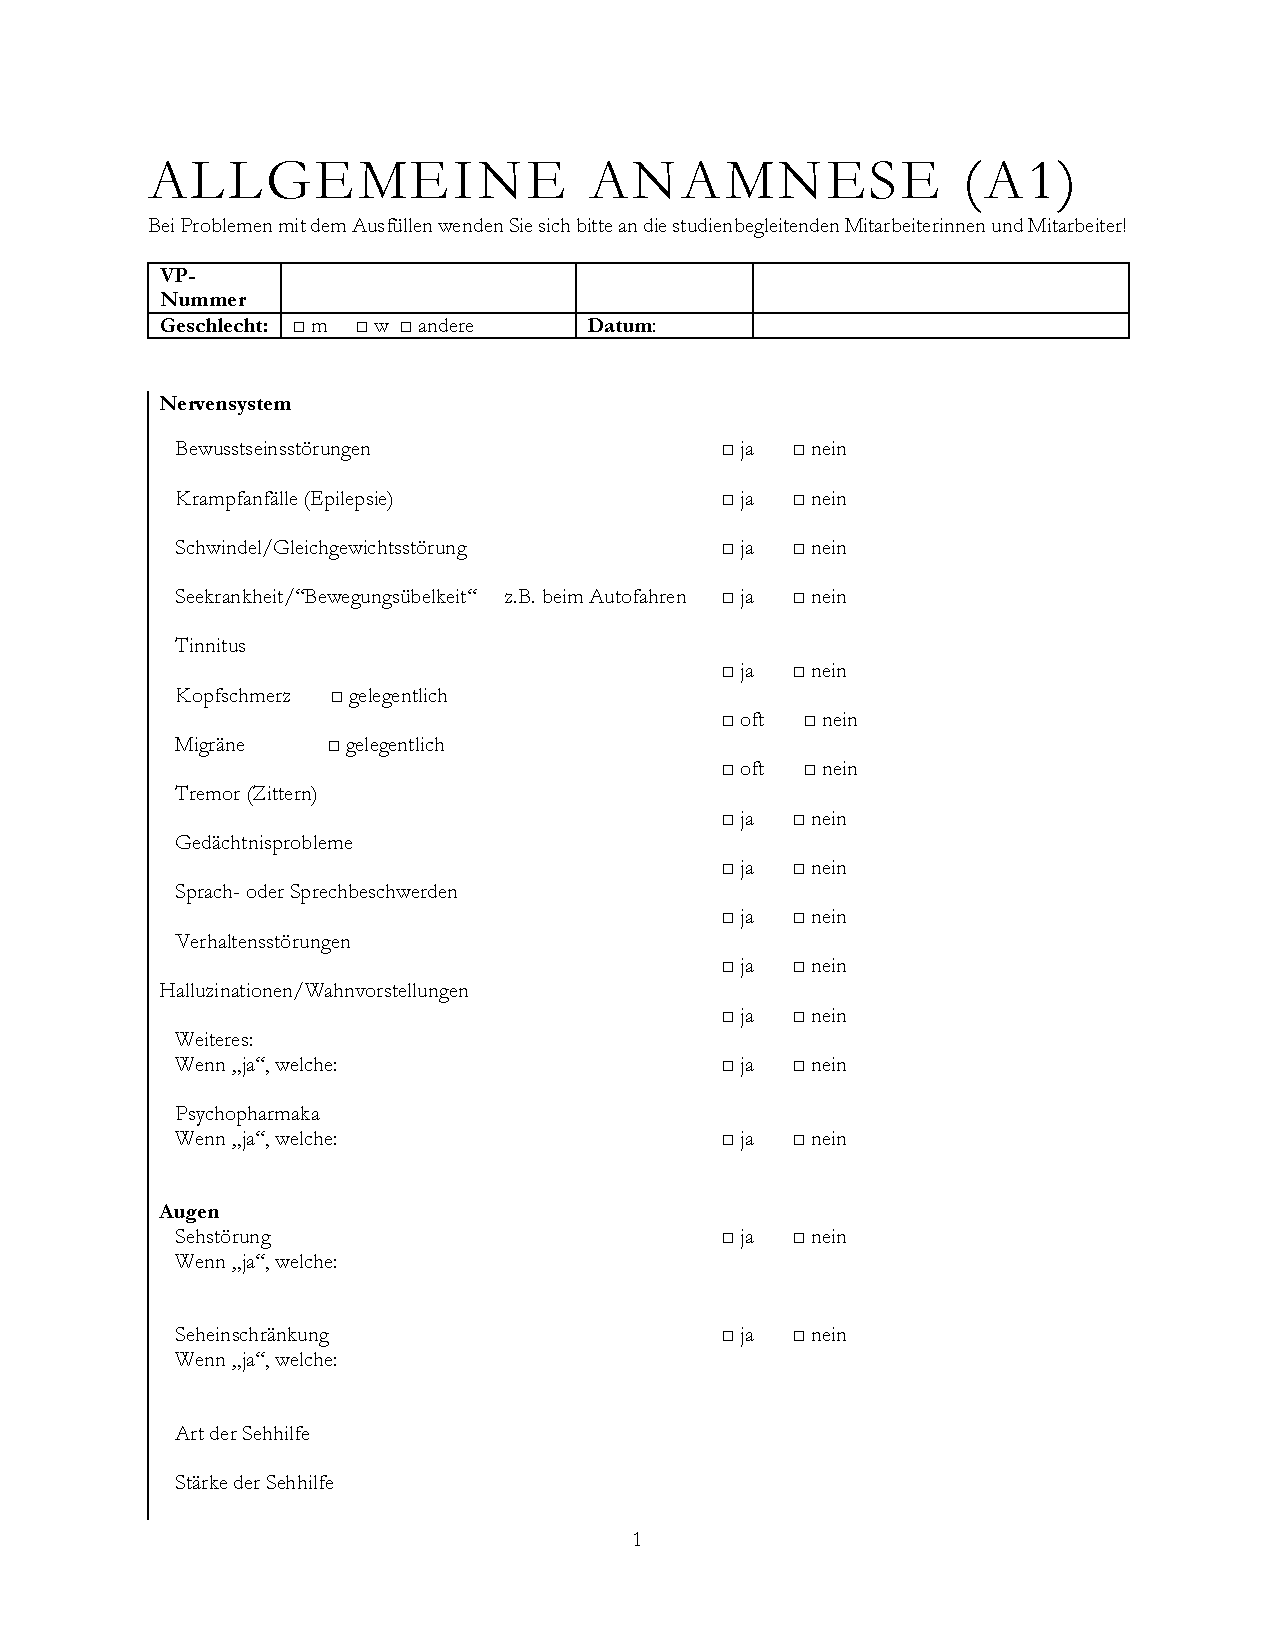
\includepdf[pages=-]{files/anamnese_VR_HumanA_German.pdf}
